%%You can delete all the comments after you have finished your document
%this sets up the defaults for the documents, 12pt font and A4 size. The article type sets this up as such as opposed to letter or memo.

%for the finer points LaTeX see https://en.wikibooks.org/wiki/LaTeX or http://tex.stackexchange.com/

\documentclass[12pt,a4paper]{article}
\usepackage{titlesec} %these are how we import packages, one helps set up footers and title layout
\usepackage{fancyhdr}

% !TEX TS-program = pdflatex
% !TEX encoding = UTF-8 Unicode
\usepackage[utf8]{inputenc} % set input encoding (not needed with XeLaTeX)
\usepackage{graphicx} % support the \includegraphics command and options

% \usepackage[parfill]{parskip} % Activate to begin paragraphs with an empty line rather than an indent

%%% PACKAGES
\usepackage{booktabs} % for much better looking tables
\usepackage{array} % for better arrays (eg matrices) in maths
\usepackage{paralist} % very flexible & customisable lists (eg. enumerate/itemize, etc.)
\usepackage{verbatim} % adds environment for commenting out blocks of text & for better verbatim
\usepackage{subfig} % make it possible to include more than one captioned figure/table in a single float
\usepackage[table,xcdraw]{xcolor}
\usepackage[toc,page]{appendix}
\usepackage{amsthm}
\usepackage[square,sort]{natbib}
\usepackage{tikz}
\usetikzlibrary{er,positioning}
\usepackage{amsmath}
\usepackage{supertabular}
\usepackage{pdfpages}
\usepackage{enumitem}
\usepackage{longtable}
\usepackage{rotating}
\usepackage{pdflscape}
\usepackage{pdfpages}
\usepackage{verbatim}
\usepackage{pgfplots}
\usepackage[ruled,vlined]{algorithm2e}
\usepackage{algorithmic}
\usepackage{blkarray}
\usepackage{multirow}
\usepackage{tcolorbox}
\usepackage[cache=false]{minted}
\usepackage{dirtree}

\graphicspath{{./img/}}

\theoremstyle{definition}
\newtheorem{definition}{Definition}[section]

\newtheorem{theorem}{Theorem}
% These packages are all incorporated in the memoir class to one degree or another...

%header and footer settings
\pagestyle{fancyplain}
\fancyhf{}
\renewcommand{\headrulewidth}{0.5pt}
\renewcommand{\footrulewidth}{0.5pt}
\setlength{\headheight}{15pt}
\fancyhead[L]{Marcin Szczot - 40180425}
\fancyhead[R]{ SOC10101 Honours Project}
\fancyfoot[L]{}
\fancyfoot[C]{\thepage}

%set better section layout
\makeatletter
\renewcommand\subsection{\@startsection {subsection}{1}{2mm} % name, level, indent
                               {3pt plus 2pt minus 1pt} % before skip
                               {3pt plus 0pt} % after skip
                               {\normalfont\bfseries}}
\renewcommand\subsubsection{\@startsection {subsubsection}{2}{4mm} % name, level, indent
                               {3pt plus 2pt minus 1pt} % before skip
                               {3pt plus 0pt} % after skip
                               {\normalfont\bfseries}}
\makeatother
\makeatletter
\renewcommand\section{\@startsection {section}{1}{0mm} % name, level, indent
                               {4pt plus 2pt minus 1pt} % before skip
                               {4pt plus 0pt} % after skip
                               {\bfseries}}
                            
\renewcommand\paragraph{\@startsection {paragraph}{3}{6mm} % name, level, indent
                     	{3pt plus 2pt minus 1pt} % before skip
                     	{3pt plus 0pt} % after skip
                     	{\bfseries}}
\makeatother

\setcounter{secnumdepth}{4}
\setcounter{tocdepth}{4}


\pgfplotstableread[row sep=\\,col sep=&]{
	Solver & Time & Score \\
	argmat-sat & 369.6084 & 1065 \\
	pyglaf & 391.1673 & 909 \\
	cegartix & 548.225 & 898 \\
	goDIAMOND & 691.1238 & 724 \\
	conarg & 552.8406 & 649 \\
	argmat-mpg & 472.5955 & 618 \\
	ArgTools & 1224.124 & 67 \\
	CoQuiAAS & 277.9286 & -305 \\
	gg-sts & 581.4469 & -1325 \\ 
}\stageResults

\pgfplotstableread[row sep=\\,col sep=&]{
	    Solver & Time & Score\\
	pyglaf & 222.2444 & 1226 \\
	cegartix & 263.6557 & 1181 \\
	argmat-sat & 245.8243 & 1167\\
	argmat-dvisat & 291.0360 & 1147\\
	CoQuiAAS & 186.4464 & 1134\\
	argmat-mpg & 316.5906 & 1125\\
	goDIAMOND & 224.2296 & 1110\\
	heureka & 	272.8588 & 1021\\
	conarg & 	184.4099 & 1017\\
	ArgTools & 553.4805 & 935\\
	ArgSemSAT & 388.0886 & 905\\
	EqArgSolver & 142.1794 & 422\\
	argmat-clpb & 1270.5737 & 40\\
	gg-sts & 	149.6766 & -1160\\
}\completeResults

\pgfplotstableread[row sep=\\,col sep=&]{
	Solver	 & 	Time	 & 	Score	\\
	ArgSemSAT	 & 	269.0961143	 & 	1146	 \\
	argmat-sat	 & 	283.6564857	 & 	1139	 \\
	pyglaf	 & 	225.2380857	 & 	1120	 \\
	argmat-dvisat	 & 	358.0394429	 & 	1075	 \\
	cegartix	 & 	357.13085	 & 	1075	 \\
	goDIAMOND	 & 	360.4056786	 & 	1014	 \\
	ArgTools	 & 	569.3684643	 & 	898	 \\
	conarg	 & 	502.1910786	 & 	773	 \\
	argmat-mpg	 & 	551.9100714	 & 	745	 \\
	heureka	 & 	571.0247143	 & 	745	 \\
	EqArgSolver	 & 	175.8627072	 & 	652	 \\
	ASPrMin	 & 	84.42593573	 & 	285	 \\
	ChimaerArg	 & 	41.35408573	 & 	92	 \\
	CoQuiAAS	 & 	259.1468286	 & 	-863	 \\
	gg-sts	 & 	323.0009643	 & 	-1107	 \\	
}\preferredResults

\pgfplotstableread[row sep=\\,col sep=&]{
	Solver	&	Time	&	Score	\\
	pyglaf	&	90.1213643	&	585	\\
	argmat-dvisat	&	178.3911714	&	493	\\
	argmat-sat	&	193.0512643	&	477	\\
	goDIAMOND	&	244.3234	&	414	\\
	cegartix	&	108.8148357	&	368	\\
	ArgTools	&	348.1760357	&	268	\\
	argmat-mpg	&	345.6741357	&	217	\\
	conarg	&	383.2702572	&	181	\\
	CoQuiAAS	&	84.07600715	&	-794	\\
	gg-sts	&	183.6329357	&	-1050	\\
}\idealResults

\pgfplotstableread[row sep=\\,col sep=&]{
	Solver	&	Time	&	Score	\\
	pyglaf	&	228.9274429	&	1183	\\
	goDIAMOND	&	279.1122214	&	1143	\\
	argmat-sat	&	276.8502	&	1129	\\
	cegartix	&	354.8398858	&	1102	\\
	argmat-mpg	&	419.0768643	&	1073	\\
	argmat-dvisat	&	363.1061	&	1039	\\
	conarg	&	446.6884286	&	1002	\\
	heureka	&	389.9640072	&	938	\\
	ArgSemSAT	&	355.2810214	&	888	\\
	ArgTools	&	408.3974	&	687	\\
	EqArgSolver	&	175.2068357	&	558	\\
	argmat-clpb	&	1362.999786	&	135	\\
	ChimaerArg	&	28.23509285	&	-220	\\
	CoQuiAAS	&	347.5605429	&	-299	\\
	gg-sts	&	229.54905	&	-1193	\\
}\stableResults

\pgfplotstableread[row sep=\\,col sep=&]{
	Solver & Time & Score \\
	argmat-sat & 256.0897 & 1164 \\
	ArgSemSAT & 282.8889 & 1113 \\
	cegartix & 320.8204 & 1091 \\
	pyglaf & 305.5463 & 1047 \\
	goDIAMOND & 379.4291 & 1032 \\
	argmat-mpg & 475.7026 & 755 \\
	conarg & 495.7143 & 668 \\
	ArgTools & 617.3107 & 268 \\
	gg-sts & 255.5661 & -1321 \\
	CoQuiAAS & 224.1309 & -1642 \\ 
}\semiStableResults

\pgfplotstableread[row sep=\\,col sep=&]{
	Solver & Time & Score \\
	ArgSemSAT & 269.0961143 & 1146 \\
	argmat-sat & 283.6564857 & 1139 \\
	pyglaf & 225.2380857 & 1120 \\
	argmat-dvisat & 358.0394429 & 1075 \\
	cegartix & 357.13085 & 1075 \\
	goDIAMOND & 360.4056786 & 1014 \\
	ArgTools & 569.3684643 & 898 \\
	conarg & 502.1910786 & 773 \\
	argmat-mpg & 551.9100714 & 745 \\
	heureka & 571.0247143 & 745 \\
	EqArgSolver & 175.8627072 & 652 \\
	ASPrMin & 84.42593573 & 285 \\
	ChimaerArg & 41.35408573 & 92 \\
	CoQuiAAS & 259.1468286 & -863 \\
	gg-sts & 323.0009643 & -1107 \\	
}\preferredResults

\pgfplotstableread[row sep=\\, col sep=&]{
Args & attacks & Time \\
2/1 & 1 & 0.000087 \\
13/17 & 17 & 0.1819 \\
15/5 & 5 & 0.9173 \\
15/2 & 2 & 1.8042 \\
19/15 & 15 & 238.425 \\
}\aliasvResults

\definecolor{grey}{RGB}{211,211,211}

%this starts the document
\begin{document}

%you can import other documents into your main one, these layout the Title and Declarations on its own page.
%you might need to change these to \ if your on Microsoft Windows.
\newcommand{\HRule}{\rule{\linewidth}{0.5mm}}

\begin{titlepage}
	\begin{center}

	\HRule \\[0.4cm]
    	{\Large \bfseries Computing Abstract Argumentation Semantics\par}
	\vspace{0.2cm}
	\HRule \\[1.5cm]

	
    	\vspace{3cm}
	\begin{minipage}{0.4\textwidth}
	\begin{center} \large
        \emph{}\\
        	Marcin Szczot - 40180425
				
   	 \end{center}
    	\end{minipage}
	
	\vspace{2cm}
    	\begin{minipage}{1\textwidth}
    	\begin{center} \large
        
		Submitted in partial fulfilment of \\
		the requirements of Edinburgh Napier University \\
		for the Degree of \\
        	BEng (Hons) Software Engineering
    	\end{center}
    	\end{minipage}

    	\vfill

    	% Bottom of the page
	\begin{minipage}{1\textwidth}
    	\begin{center} \large
		School of Computing
    	\end{center}
    	\end{minipage}
	
	\vspace{1cm}
    	{\large \today}


	\end{center}
\end{titlepage}
%{\large Submitted in partial fulfilment of the requirements of Edinburgh Napier University for the Degree of }

\section*{Authorship Declaration}
\vspace{0.5cm}
\begin{flushleft}
I, (Insert Name eg. Norman Stanley Fletcher), confirm that this dissertation and the work presented in it are my own achievement.\newline

Where I have consulted the published work of others this is always clearly attributed;\newline

Where I have quoted from the work of others the source is always given. With the exception of such quotations this dissertation is entirely my own work;\newline

I have acknowledged all main sources of help; \newline

If my research follows on from previous work or is part of a larger collaborative research project I have made clear exactly what was done by others and what I have contributed myself;\newline

I have read and understand the penalties associated with Academic Misconduct.\newline

I also confirm that I have obtained informed consent from all people I have involved in the work in this dissertation following the School's ethical guidelines.\newline
\end{flushleft}

\begin{flushleft} \large
\emph{Signed:} \\
\end{flushleft}

\vspace{.5cm}

\begin{flushleft} \large
\emph{Date:} \\
\end{flushleft}

\vspace{.5cm}

\begin{flushleft} \large
\emph{Matriculation no: }  \\
\end{flushleft}
\pagebreak

\section*{Data Protection Declaration}
\vspace{0.5cm}
\begin{flushleft}
Under the 1998 Data Protection Act, The University cannot disclose your grade to an unauthorised person. However, other students benefit from studying dissertations that have their grades attached. \newline

\vspace{0.5cm}

Please sign your name below one of the options below to state your preference.\newline
\vspace{0.5cm}

The University may make this dissertation, with indicative grade, available to others.\newline
\vspace{3cm}


The University may make this dissertation available to others, but the grade may not be disclosed.\newline
\vspace{3cm}


The University may not make this dissertation available to others.\newline
\end{flushleft}


\pagebreak

%LaTeX let you define the abstract separately so it wont get sucked into the main document.
\begin{abstract}
\documentclass[../Dissertation.tex]{subfiles}

\begin{document}
	
\end{document}
\end{abstract}
\pagebreak

\tableofcontents % is generated for you
\newpage

\listoftables
%generated in same way as figures
\newpage

\listoffigures
%you may have captions such as equations, listings etc they should all appear as required
%these are done for you as long as you use \begin{figure}[placement settings] .. bla bla ... \end{figure}
\newpage

\section*{Acknowledgements}
Insert acknowledgements here
\subsection*{}
	I would like to thank my cat, dog and family.
\newpage

%-------------------------------------------------------------------------------
% Main content 
%-------------------------------------------------------------------------------
\section{Introduction} \label{section:introduction}
This is my test \cite{dung1995acceptability}

\section{Literature \& Technical Review} \label{section:literatureReview}
\subsection{Abstract Argumentation} \label{abstractArgumentation}
Argumentation framework has been introduced by \citet{dung1995} and is central to the theory of abstract argumentation \citep{baroni2011introduction}. It is defined as a pair of a set of arguments, and a binary relation representing the attack relationship between arguments \citep{dung1995}. 

\theoremstyle{definition}
\begin{definition}{Argumentation Framework}
\label{AFdef}\\
An argumentation framework is a pair \textit{AF} = $<$\textit{AR, attacks}$>$ in which \textit{AR} is a set of finite arguments, and \textit{attacks} is a binary relation on \textit{AR}, hence \textit{attacks} $\subseteq$ \textit{AR} $\times$ \textit{AR}, where \textit{AR} $\times$ \textit{AR} = \{(\textit{a}, \textit{b}) $\vert$ \textit{a} $\in$ \textit{AR} and \textit{b} $\in$ \textit{AR}\}
\end{definition}

In definition \ref{AFdef}, \textit{AR} represents a set of arguments and \textit{attacks} represents set of pairs of arguments (\textit{a, b}), where (\textit{a, b}) $\in$ \textit{attacks}. Each pair of arguments in \textit{attacks} represents two arguments being in conflict. Hence, the arguments \textit{a} and \textit{b} from definistion \ref{AFdef} are in conflict and the meaning of \textit{attacks(a, b)} is that \textit{a} attacks \textit{b}. Based on this definition, we can conclude that the set of arguments \textit{AR} is conflict-free if and only if there are no arguments \textit{a} and \textit{b} in \textit{AR} such that \textit{a} attacks \textit{b}, or \textit{b} attacks \textit{a} \citep{dung1995}.

The argumentation framework can be represented as directed graph where the nodes represent abstract arguments and edges the attack relation. This can be seen in figure \ref{fig:argumentationFrameworkFigure}, where argument \textit{a} attacks argument \textit{b}, which in turn attacks argument \textit{c}. \textit{C} is also attacked by argument \textit{d}.
\newpage
\begin{figure}[h]
\tikzset{
    main/.style={draw, rectangle, rounded corners, minimum height=1cm, minimum width=4.5cm},
    arrow/.style={thick,<-,>=stealth}
}
\centering
\begin{tikzpicture}[auto,node distance=1.5cm]
	\node[draw=none,fill=none](a){a};
	\node[draw=none,fill=none][right=of a](b){b};
	\node[draw=none,fill=none][right=of b](c){c};
	\node[draw=none,fill=none][right=of c](d){d};	
  	%%% ARROWS %%%
  	\draw[arrow](b) -- (a);
  	\draw[arrow](c) -- (b);
  	\draw[arrow](c) -- (d);
\end{tikzpicture}
\caption{Argumentation Framework \ref{fig:argumentationFrameworkFigure}}
\label{fig:argumentationFrameworkFigure}
\end{figure}
 
Example of the argumentation framework can also be presented using the following example from \citet{konolige1988defeasible}:
\begin{quote}
Suppose Ralph normally goes fishing on Sundays, but on the Sunday which is
Mother’s day, he typically visits his parents. Furthermore, in the spring of each
leap year, his parents take a vacation, so that they cannot be visited.
\end{quote}
If we assume it is Sunday, Mother's day and a leap year, then three arguments can be formulated from the extract above:
\begin{enumerate}[label=\Alph*]
	\item{Ralph goes fishing because it is Sunday.}
	\item{Ralph does not go fishing because it is Mother's day, hence he visits his parents.}
	\item{Ralph does not go visit his parents, because it is a leap year. Hence, they are on vacation.}
\end{enumerate}
In this example argument \textit{B} attacks argument \textit{A} and argument \textit{C} attacks argument \textit{B}. Since argument \textit{C} can be justified, as it is not attacked, then \textit{B} is defeated and does no longer form a reason against \textit{A}. We can say that argument \textit{C} reinstates argument \textit{A} \citep{caminada2004sake}.


Dung in his paper \citep{dung1995} has also defined notions of \textit{acceptable} and \textit{admissible} arguments, which are as follow:

\begin{definition}{Acceptable argument}
\label{AcceptableArgDef}\\
An argument \textit{a} $\in$ \textit{AR} is said to be \textit{acceptable} with respect to set \textit{S} $\subseteq$ \textit{AR} if and only if for each argument \textit{b} $\in$ \textit{AR} such that (\textit{b}, \textit{a}) $\in$ \textit{attacks}, there are some arguments \textit{c} $\in$ \textit{S} such that (\textit{c}, \textit{b}) $\in$ \textit{attacks}
\end{definition}

Hence it can be said that the argument from given argumentation framework is acceptable with respect to the set only if it is either conflict free, or there exists an argument from the same set that defends given argument. Based on the definition \ref{AcceptableArgDef}, definition of \textit{admissible} set can be concluded:

\begin{definition}{Admissible argument} \label{admissibleArgument}
\label{AdmissibleArgDef}\\
A conflict-free set of arguments \textit{S} is \textit{admissible} if and only if each argument in \textit{S} is acceptable with respect to \textit{S}.
\end{definition}

That means that the set of arguments can be described as admissible only if it is conflict-free and all of its arguments can be defended by other arguments from that set. Both definitions have important role in defining the semantics of abstract argumentation. An argumentation semantics can be described as the formal definition of a method (declarative or procedural) ruling the argument evaluation process \citep{baroni2009semantics}. Hence, they are used to evaluate if the arguments can be justified, by being defended by other arguments in the set, or rejected. 

There are two approaches for defining argumentation semantics: extension and labelling based. In the extension-based approach semantic definition specifies how to derive from an argumentation framework a set of extensions, where an extension \textit{E} of an argumentation framework $<$\textit{AR, attacks}$>$ is simply a subset of \textit{AR}, intuitively representing a set of arguments which can “survive together” or are “collectively acceptable” \citep{baroni2009semantics}. On the other hand labelling-based approach defines how the arguments can be labelled based on the predefined set of labels. Labels define the possible states of argument and those are as follow: 
\begin{itemize}
	\item \textit{in}, when argument can be justified, 
	\item \textit{out} when argument is rejected, and 
	\item \textit{undecided} to any other argument.
\end{itemize}

As shown by Modgil and Caminada, label-based approach is suitable for characterizing argumentation semantics \citep{modgil2009proof}.
\subsection{Argumentation Semantics}
\label{sec:argumentationSemantics}


The original concept of abstract argumentation semantics included complete, stable, preferred and grounded extensions \citep{dung1995}, which was extended by stage \citep{verheij1996two}, ideal \citep{dung2007computing}, and semi-stable \citep{caminada2006semi} semantics. All the sematics are based around the definitions of acceptable and admissible arguments. Definitions of the original semantics as described by \citet{dung1995} are as follow: 

\begin{definition}{Preferred Extension}
\label{def:preferredExtension}\\
A \textit{preferred extension} of an argumentation framework \textit{AF} is a maximal (with respect to set inclusion) admissible set of \textit{AF}.
\end{definition}


From the definition \ref{def:preferredExtension} it can be seen that the preferred extension is the largest set that is able to defend itself from attacks. If we consider example \ref{fig:af1} we can see that the extension \textit{$E_{PR}$} = \{\{a,c\}, \{b\}\}. Argument \textit{c} is attacked by argument \textit{b}, which in turn is defeated by \textit{a}, hence \textit{a} and \textit{c} are preferred extension. Furthermore, \textit{b} is attacked by \textit{a}, but it defends itself. Hence argument \textit{b} is also preferred extension.

\begin{figure}[h]
\tikzset{
    main/.style={draw, rectangle, rounded corners, minimum height=1cm, minimum width=4.5cm},
    arrow/.style={thick,<-,>=stealth}
}
\centering
\begin{tikzpicture}[auto,node distance=1.5cm]
	\node[draw=none,fill=none](c){c};
	\node[draw=none,fill=none][right=of c](b){b};
	\node[draw=none,fill=none][right=of b](a){a};	
  	%%% ARROWS %%%
  	\draw[thick,<-,>=stealth,transform canvas={yshift=0.5em}](b) -- (a);
  	\draw[arrow](c) -- (b);
  	\draw[thick,<-,>=stealth,transform canvas={yshift=-0.2em}](a) -- (b);
\end{tikzpicture}
\caption{Argumentation Framework \ref{fig:af1}}
\label{fig:af1}
\end{figure}

\begin{definition}{Stable Extension}
\label{def:stableExtension}\\
A \textit{conflict-free} set of arguments \textit{S} is called a \textit{stable extension} if and only if \textit{S} attacks each argument which does not belong to \textit{S}.
\end{definition}

Stable extension has more aggressive approach than preferred extension. As in definition \ref{def:stableExtension}, the extension needs to attack all arguments that are not included in it. Based on argumentation framework from example \ref{fig:af1}, the stable extension \textit{$E_{ST}(AF_{\ref{fig:af1}})$} = \{\{a,c\}, \{b\}\}, which is the same as for preferred extension. This is because argument \textit{a} attacks \textit{b}, hence \textit{a} and \textit{c} are included, and argument \textit{b} attack both arguments \textit{a} and \textit{c}. Looking at more complex example in figure \ref{fig:af2}, three stable extensions can be identified as follow \textit{$E_{ST}(AF_{\ref{fig:af2}})$} = \{\{a,c\}, \{a,d\}, \{b,d\}\}.

\begin{figure}[h]
\tikzset{
    main/.style={draw, rectangle, rounded corners, minimum height=1cm, minimum width=4.5cm},
    arrow/.style={thick,<-,>=stealth}
}
\centering
\begin{tikzpicture}[auto,node distance=1.5cm]
	\node[draw=none,fill=none](c){c};
	\node[draw=none,fill=none][left=of c](d){d};
	\node[draw=none,fill=none][right=of c](b){b};
	\node[draw=none,fill=none][right=of b](a){a};	
  	%%% ARROWS %%%
  	\draw[thick,<-,>=stealth,transform canvas={yshift=0.5em}](b) -- (a);
  	\draw[arrow](c) -- (b);
  	\draw[thick,<-,>=stealth,transform canvas={yshift=-0.2em}](a) -- (b);
  	\draw[thick,<-,>=stealth,transform canvas={yshift=-0.2em}](c) -- (d);
  	\draw[thick,<-,>=stealth,transform canvas={yshift=0.5em}](d) -- (c);
\end{tikzpicture}
\caption{Argumentation Framework \ref{fig:af2}}
\label{fig:af2}
\end{figure}

\citet{dung1995} in his paper also defined a skeptical semantics known as grounded extension. This extension is defined in terms of \textit{characteristic function}, which in turn is defined as:

\begin{definition}{Characteristic Function}
\label{def:characteristicFunction}\\
The \textit{characteristic function}, denoted by \textit{F\textsubscript{AF}}, of an argumentation framework \textit{AF} = $<$\textit{AR, attacks}$>$ is defined as follows:
\[F_{AF}:2^{AR} \rightarrow 2^{AR}\]
\[F_{AF}(S)=\{A| \text{A is acceptable with respect to S} \}\]
\end{definition}

\begin{definition}{Grounded Extension}
\label{def:groundedExtension}\\
The \textit{grounded extension} of an argumentation framework \textit{AF}, denoted by \textit{GE\textsubscript{AF}}, is the least fixed point of \textit{F\textsubscript{AF}}.
\end{definition}

Based on the definition of characteristic function and grounded extension it can be noted that the grounded extension has very restrictive approach for its computation, as it only includes the arguments whose defence is "rooted" in initial unattacked argument \citep{baroni2009semantics}. Hence, the grounded extension from figure \ref{fig:af3} is \textit{$E_{GR}(AF_{\ref{fig:af3}})$} = \{\{a,c\}\}. Starting from argument \textit{a}, as it is the only unattacked argument, we reject argument \textit{b} and include \textit{c}. Furthermore, argument \textit{d} is being rejected, as it is attacked by \textit{c}. Although, argument \textit{e} attacks argument \textit{f}, it is attacked by \textit{f} as well. Hence, it cannot be part of grounded extension.

\begin{figure}[h]
\tikzset{
    main/.style={draw, rectangle, rounded corners, minimum height=1cm, minimum width=4.5cm},
    arrow/.style={thick,<-,>=stealth}
}
\centering
\begin{tikzpicture}[auto,node distance=1.5cm]
	\node[draw=none,fill=none](a){a};
	\node[draw=none,fill=none][right=of a](b){b};
	\node[draw=none,fill=none][right=of b](c){c};	
	\node[draw=none,fill=none][right=of c](d){d};
	\node[draw=none,fill=none][right=of d](e){e};
	\node[draw=none,fill=none][right=of e](f){f};			
  	%%% ARROWS %%%
  	\draw[arrow](b) -- (a);
  	\draw[arrow](c) -- (b);
  	\draw[arrow](d) -- (c);
  	\draw[arrow](e) -- (d);
  	\draw[thick,<-,>=stealth,transform canvas={yshift=-0.2em}](e) -- (f);
  	\draw[thick,<-,>=stealth,transform canvas={yshift=0.5em}](f) -- (e);
\end{tikzpicture}
\caption{Argumentation Framework \ref{fig:af3}}
\label{fig:af3}
\end{figure}

\begin{definition}{Complete Extension}
\label{def:completeExtension}\\
An admissible set \textit{S} of arguments is called \textit{complete exension} if and only if each argument which is acceptable with respect to \textit{S}, belongs to \textit{S}.
\end{definition}

Complete extension is defined as a set which is able to defend itself and includes all arguments it defends \citep{baroni2009semantics}. Based on this, we can see that there are three complete extensions in figure \ref{fig:af1}, and those are \textit{$E_{CO}(AF_{\ref{fig:af1}})$} = \{$\emptyset$, \{a,c\}, \{b\}\}. With a more complex argumentation framework in figure \ref{fig:af2}, it can be seen that the complete extension will definitely include empty set, as there are no initial arguments, argument \textit{a}, as it does not defend argument \textit{c} from \textit{d}, and argument \textit{d}, as it only defends itself. Furthermore, \textit{b} attacks \textit{c}, the only attacked of argument \textit{d}, hence set \{b,d\} is a complete extension as well. Additionally, sets \{a,c\} and \{a,d\} are also compltete extensions as both of them are admissible. Hence, the complete extension is \textit{$E_{CO}(AF_{\ref{fig:af2}})$} = \{$\emptyset$, \{a\}, \{d\}, \{a,c\}\, \{a,d\}, \{b,d\}\}.

As mentioned earlier, \citet{dung1995} semantics were further extended with additional semantics. Their definitions are as follow: 

\begin{definition}{Semi-stable Extension}
\label{def:semiStableExtension}\\
Let (\textit{AR}, \textit{attacks}) be an argumentation framework and \textit{Args} $\subseteq$ \textit{AR}. \textit{Args} is called \textit{semi-stable extension} if and only if \textit{Args} is a complete extension where \textit{Args} $\cup$ \textit{$Args^+$} is maximal.
\end{definition}

The idea for semi-stable extension consist in expressing a definite opinion on the largest possible set of arguments, while restricting as much as possible those which are left undecided \citep{baroni2011introduction}, where labelling has been used. Hence, the stable-extension in argumentation framework in figure \ref{fig:af4} is \textit{$E_{SST}(AF_{\ref{fig:af4}})$} = \{\{b,d\}\}, which is also a preferred extension.

\begin{figure}[h]
\tikzset{
    main/.style={draw, rectangle, rounded corners, minimum height=1cm, minimum width=4.5cm},
    arrow/.style={thick,<-,>=stealth}
}
\centering
\begin{tikzpicture}[auto,node distance=1.5cm]
	\node[draw=none,fill=none](a){a};
	\node[draw=none,fill=none][right=of a](b){b};
	\node[draw=none,fill=none][right=of b](c){c};	
	\coordinate[right=0.75cm of c](coordinate);
	\node[draw=none,fill=none][above =0.5cm of coordinate](d){d};
	\node[draw=none,fill=none][below =0.5cm of coordinate](e){e};		
  	%%% ARROWS %%%
  	\draw[thick,<-,>=stealth,transform canvas={yshift=-0.2em}](a) -- (b);
  	\draw[thick,<-,>=stealth,transform canvas={yshift=0.5em}](b) -- (a);
  	\draw[arrow](c) -- (b);
	\draw[thick, -latex] (c.north) to [bend left=45](d.west);
	\draw[thick, -latex] (d.east) to [bend left=90](e.east);
	\draw[thick, -latex] (e.west) to [bend left=45](c.south);
\end{tikzpicture}
\caption{Argumentation Framework \ref{fig:af4}}
\label{fig:af4}
\end{figure}

\begin{definition}{Ideal Extension}
\label{def:idealExtension}\\
The \textit{ideal extension} is the greatest with respect to set inclusion admissible set that is a subset of each preferred extension.
\end{definition}

By its definition the ideal extension satisfies I-maximality and admissibility principles \citep{baroni2009semantics}. The I-maximiality is a property of the set of extensions, without reference to any generic criterion \citep{dunne2006computational}. It is defined as:

\begin{definition}{I-maximality}
\label{def:IMaximality}\\
A set of extensions \textit{E} is I-maximal if and only if $\forall$\textit{$E_1$}, \textit{$E_2$} $\in$ \textit{E}, if \textit{$E_1$} $\subseteq$ \textit{$E_2$} then \textit{$E_1$} = \textit{$E_2$}.
\end{definition}

Perhaps, the ideal semantics can be best explained using the notion of a judgement aggregation context intoduced by \citet{caminada2011judgment}. Given an argumentation framework, if we assume a group of people who all try to accept as much as possible the sets of arguments they all agree on needs to be examined and checked whether this position is still defensible. However, if they are not defensible some of the arguments needs to be abstained from instead of accepting or rejecting them until it becomes defensible. The result is the ideal extension \citep{baroni2011introduction}.

\begin{definition}{Stage Extension}
\label{def:stageExtension}\\
Let (\textit{AR}, \textit{attacks}) be an argumentation framework. A \textit{stage extension} conflict-free set \textit{Args} $\subseteq$ \textit{AR}, where \textit{Args} $\cup$ \textit{$Args^+$} is maximal with respect to set inclusion among all conflict-free sets.
\end{definition}

Stage extension introduced by \citet{verheij1996two} can also be explained in terms of labelling. It is a conflict-free extension where number of arguments labeled \textit{undec} is minimal. 
\newline

\begin{figure}[h]
\tikzset{
    main/.style={draw, rectangle, rounded corners, minimum height=1cm, minimum width=4.5cm},
    arrow/.style={thick,<-,>=stealth}
}
\centering
\begin{tikzpicture}[auto,node distance=1.5cm]
	\node[main](1){Complete Semantics};
	\coordinate[below=of 1](c);
  	\node[main](2)[left=of c]{Grounded Semantics};
  	\node[main](3)[right=of c]{Ideal Semantics};
  	\node[main](4)[below=of c]{Preferred Semantics};
  	\node[main](5)[below=of 4]{Semi-Stable Semantics};
  	\node[main](7)[below=of 5]{Stable Semantics};  	
  	\node[main](6)[right=of 7]{Stage Semantics};
  	%%% ARROWS %%%
  	\draw[arrow](1) -- (2) node[midway] {is a};
  	\draw[arrow](1) -- (3) node[midway] {is a};
  	\draw[arrow](1) -- (4) node[midway] {is a};
  	\draw[arrow](4) -- (5) node[midway] {is a};
  	\draw[arrow](5) -- (7) node[midway] {is a};  	
  	\draw[arrow](6) -- (7) node[midway] {is a};
\end{tikzpicture}
\caption{Relations of semantics}
\label{fig:semanticsRelations}
\end{figure}

Above semantics can be used to decide whether a given argument, or set of arguments can be accepted in terms of set inclusion.  Based on the definitions a number of inclusions between the sets can be conluded. Those are:
\begin{itemize}
	\item{Grounded extension is the smallest complete extension}
	\item{Every preferred extesion is also complete}
	\item{Every stable extension is also semi-stable and stage extension}
\end{itemize}
Furthermore, it can be seen that the complete extension provides the link between preferred extension (credulous semantic), and grounded extension (skeptical smenatics) \citep{dung1995}. It can also be concluded seen that the maximal complete extension is also maximal admissible set. On the other hand the grounded extension is determined by the minimal complete extension \citep{gaggl2009solving}. The relations between the semantics can be seen in figure \ref{fig:semanticsRelations}.


%sceptical and credulous semantics
%sceptical and credulous acceptance of argument
Additional notion of credulous and sceptical semantics has been introduced. Usually, a credulous semantics is intended to capture as much information as possible \citep{dix1995non}, while skeptical makes less committed choices about the justification of the arguments \citep{baroni2007comparing}. As mentioned previosly grounded semantic is a good example of skeptical extension as it always yields exactly one extension, and this extension is admissible \citep{caminada2007comparing}.

Furthermore, argument can be defined as credulous or skeptical in terms of its acceptability. As describe by \citet{arieli2015conflict} an argument \textit{a} $\in$ \textit{Args} is credulously accepted by one type of semantics only if it belongs to some of the semantic extensions of a given argumentation framework. On the other hand, the argument \textit{b} is skeptically accepted by the semantic if it belongs to all of its extensions of a given argumentation framework. This can be represented using argumentation framework \ref{fig:af5}. It has 5 complete extensions: $\emptyset$, {b}, {e}, {b, e}, {a, c, e}, however none of the arguments is skeptically accepted, while \textit{a}, \textit{b}, \textit{c} and \textit{e} are credulously accepted. On the other hand, \{\textit{b, e}\} and \{\textit{a, c, e}\} are preferred, stable, semi-stable and stage extensions of argumentation framework \ref{fig:af5}. It can be seen that only argument \textit{e} is skeptically accepted for all those semantics, while \textit{a}, \textit{b} and \textit{c} are credulously accepted.

\begin{figure}[h]
\tikzset{
    main/.style={draw, rectangle, rounded corners, minimum height=1cm, minimum width=4.5cm},
    arrow/.style={thick,<-,>=stealth}
}
\centering
\begin{tikzpicture}[auto,node distance=1.5cm]
	\node[draw=none,fill=none](a){a};
	\node[draw=none,fill=none][right=of a](b){b};
	\node[draw=none,fill=none][right=of b](c){c};	
	\node[draw=none,fill=none][right=of c](d){d};	
	\coordinate[right=0.75cm of d](coordinate);
	\node[draw=none,fill=none][above =0.5cm of coordinate](e){e};
	\node[draw=none,fill=none][below =0.5cm of coordinate](f){f};		
  	%%% ARROWS %%%
  	\draw[thick,<-,>=stealth,transform canvas={yshift=-0.2em}](a) -- (b);
  	\draw[thick,<-,>=stealth,transform canvas={yshift=0.5em}](b) -- (a);
  	\draw[arrow](c) -- (b);
  	\draw[arrow](d) -- (c);
	\draw[thick, -latex] (d.north) to [bend left=45](e.west);
	\draw[thick, -latex] (e.east) to [bend left=90](f.east);
	\draw[thick, -latex] (f.west) to [bend left=45](d.south);
\end{tikzpicture}
\caption{Argumentation Framework \ref{fig:af5}}
\label{fig:af5}
\end{figure}
\subsection{Approaches to computing argumentation semantics} \label{approaches}

\begin{figure}[h]
	\centering
	\begin{tikzpicture}
	\begin{axis}[
	ybar,
	symbolic x coords={pyglaf, cegartix, argmat-sat, argmat-dvisat, CoQuiAAS, argmat-mpg, goDIAMOND, heureka, conarg, ArgTools, ArgSemSAT, EqArgSolver, argmat-clpb, gg-sts},
	xtick=data,
	x tick label style={rotate=90,anchor=east},
	legend style={at={(0.05,0.1)},anchor=west},
	]
	\addplot table[x=Solver,y=Score]{\completeResults};
	\addplot[draw=red,ultra thick,smooth] table[x=Solver,y=Time]{\completeResults};
	\legend{Score,Time}
	\end{axis}
	\end{tikzpicture}
	\caption{Results of Complete Extension Track from ICCMA 2017}
	\label{fig:coTrack}
\end{figure}

\begin{figure}[h]
	\centering
	\begin{tikzpicture}
	\begin{axis}[
	ybar,
	symbolic x coords={pyglaf,argmat-dvisat,argmat-sat,goDIAMOND,cegartix,ArgTools,argmat-mpg,conarg,CoQuiAAS,gg-sts
	},
	xtick=data,
	x tick label style={rotate=90,anchor=east},
	legend style={at={(0.05,0.1)},anchor=west},
	]
	\addplot table[x=Solver,y=Score]{\idealResults};
	\addplot[draw=red,ultra thick,smooth] table[x=Solver,y=Time]{\idealResults};
	\legend{Score,Time}
	\end{axis}
	\end{tikzpicture}
	
	\caption{Results of Ideal Extension Track from ICCMA 2017}
	\label{fig:idTrack}
	
\end{figure}

\begin{figure}[h]
	\centering
	\begin{tikzpicture}
	\begin{axis}[
	ybar,
	symbolic x coords={pyglaf,goDIAMOND,argmat-sat,cegartix,argmat-mpg,argmat-dvisat,conarg,heureka,ArgSemSAT,ArgTools,EqArgSolver,argmat-clpb,ChimaerArg,CoQuiAAS,gg-sts
	},
	xtick=data,
	x tick label style={rotate=90,anchor=east},
	legend style={at={(0.05,0.1)},anchor=west},
	]
	\addplot table[x=Solver,y=Score]{\stableResults};
	\addplot[draw=red,ultra thick,smooth] table[x=Solver,y=Time]{\stableResults};
	\legend{Score,Time}
	\end{axis}
	\end{tikzpicture}
	
	\caption{Results of Stable Extension Track from ICCMA 2017}
	\label{fig:stTrack}
\end{figure}


\begin{figure}[h]
	\centering
	\begin{tikzpicture}
	\begin{axis}[
	ybar,
	symbolic x coords={argmat-sat,ArgSemSAT,cegartix,pyglaf,goDIAMOND,argmat-mpg,conarg,ArgTools,gg-sts,CoQuiAAS
	},
	xtick=data,
	x tick label style={rotate=90,anchor=east},
	legend style={at={(0.05,0.1)},anchor=west},
	]
	\addplot table[x=Solver,y=Score]{\semiStableResults};
	\addplot[draw=red,ultra thick,smooth] table[x=Solver,y=Time]{\semiStableResults};
	\legend{Score,Time}
	\end{axis}
	\end{tikzpicture}
	
	\caption{Results of Semi Stable Extension Track for ICCMA 2017}
	\label{fig:ssTrack}
\end{figure}


\begin{figure}[h]
	\centering
	\begin{tikzpicture}
	\begin{axis}[
	ybar,
	symbolic x coords={argmat-sat,
		pyglaf,
		cegartix,
		goDIAMOND,
		conarg,
		argmat-mpg,
		ArgTools,
		CoQuiAAS,
		gg-sts,},
	xtick=data,
	x tick label style={rotate=90,anchor=east},
	legend style={at={(0.05,0.1)},anchor=west},
	]
	\addplot table[x=Solver,y=Score]{\stageResults};
	\addplot[draw=red,ultra thick,smooth] table[x=Solver,y=Time]{\stageResults};
	\legend{Score,Time}
	\end{axis}
	\end{tikzpicture}
	
	\caption{Results of Stage Extension Track for ICCMA 2017}
	\label{fig:stgTrack}
\end{figure}



\begin{figure}[h]
	\centering
	\begin{tikzpicture}
	\begin{axis}[
	ybar,
	symbolic x coords={ArgSemSAT,
		argmat-sat,
		pyglaf,
		argmat-dvisat,
		cegartix,
		goDIAMOND,
		ArgTools,
		conarg,
		argmat-mpg,
		heureka,
		EqArgSolver,
		ASPrMin,
		ChimaerArg,
		CoQuiAAS,
		gg-sts,},
	xtick=data,
	x tick label style={rotate=90,anchor=east},
	legend style={at={(0.05,0.1)},anchor=west},
	]
	\addplot table[x=Solver,y=Score]{\preferredResults};
	\addplot[draw=red,ultra thick,smooth] table[x=Solver,y=Time]{\preferredResults};
	\legend{Score,Time}
	\end{axis}
	\end{tikzpicture}
	
	\caption{Results of Preferred Extension Track for ICCMA 2017}
	\label{fig:prTrack}
\end{figure}

There are many ways of computing abstract argumentation semantics. As shown in section \ref{sec:argumentationSemantics}, semantic definitions can been represented in the form of extensions and labelling. Solvers use different algorithms for computing the extensions. In this section, different approaches for computing abstract argumentation semantics used in different solvers will be reviewed. \citet{solvingMethods} in his paper categorized the approaches into two groups: reduction approach and direct approach.

The idea of the reduction approach is to utilize existing technologies and approaches, which have been developed for a different purpose. Examples of those technologies are Boolean Satisfiability solvers, also known as SAT solvers, Answer-set programming or constraint satisfaction problem. Although those approaches have a benefit of ability to use the latest technologies that have been improved and optimized throughout the years, the biggest disadvantage is to reduce the original problem of the abstract argumentation semantics into other formalisms \citep{solvingMethods}.

In contrast to reduction approach, the direct approach does not exploit any existing technologies. Instead, each solution has been developed from scratch. The advantage of the direct approach is the ability to shape and tailor the algorithms specifically to the argumentation frameworks.

\subsubsection{ICCMA Introduction}

International Competition on Computational Models of Argumentation is held every 2 years, where different solvers compete on reasoning tasks in abstract argumentation frameworks. The 2017 competition results will be used throughout the project as a point of reference for benchmarking the proposed solution. The competition consist of 7 main tracks, where each track represent each semantics: complete, preferred, stable, semi-stable, stage, grounded and ideal. Furthermore, each track is divided into 4 reasoning problems, with exception for grounded and ideal extensions, where only tasks 1 and 3 are relevant \citep{ICCMA2017}:
\begin{enumerate}
	\item{Given an abstract argumentation framework, determine some extensions}
	\item{Given an abstract argumentation framework, determine all extensions}
	\item{Given an abstract argumentation framework and some argument, decide whether the given argument is credulously inferred}
	\item{Given an abstract argumentation framework and some argument, decide whether the given argument is skeptically inferred}
\end{enumerate}
Each above task consists of 350 benchmark sets divided into 5 categories of hardness from very easy to too hard and each set has a timeout limit of 10 minutes. For each benchmark set the solver can get following scores \citep{results_sildes}:
\begin{itemize}
	\item{1 point, if the output is correct}
	\item{-5 points, if the output is incorrect}
	\item{0 points otherwise, i.e. no result produced within the 10 minutes limit}
\end{itemize}
For the competition in 2017, there were a total of 16 solvers submitted to participate. Being implemented using different techniques and algorithms, ICCMA is a good starting place to compare and evaluate the approaches used by the solvers.

% Please add the following required packages to your document preamble:
% \usepackage{multirow}
\begin{table}[]
	\begin{tabular}{lll}
		\textbf{Approach}                                                      & \textbf{Solver}                      & \textbf{Winning Track}           \\ \hline \hline
		\multicolumn{1}{l|}{\multirow{6}{*}{SAT Based Approach}}      & argmat-dvisat               & Dung's Triathlon        \\ \cline{2-3} 
		\multicolumn{1}{l|}{}                                         & argmat-sat                  & Semi-stable, Stage      \\ \cline{2-3} 
		\multicolumn{1}{l|}{}                                         & ArgSem-SAT                  & Preferred               \\ \cline{2-3} 
		\multicolumn{1}{l|}{}                                         & cegartix                    &                         \\ \cline{2-3} 
		\multicolumn{1}{l|}{}                                         & GG-STS                      &                         \\ \cline{2-3} 
		\multicolumn{1}{l|}{}                                         & pyglaf                      & Complete, Ideal, Stable \\ \hline
		\multicolumn{1}{l|}{\multirow{4}{*}{CSP Based Approach}}      & argmat-clpb                 &                         \\ \cline{2-3} 
		\multicolumn{1}{l|}{}                                         & ConArg                      &                         \\ \cline{2-3} 
		\multicolumn{1}{l|}{}                                         & CoQuiAAS                    & Grounded                \\ \cline{2-3} 
		\multicolumn{1}{l|}{}                                         & argmat-mpg                    &     \\
		 \hline
		\multicolumn{1}{l|}{\multirow{2}{*}{ASP Based Approach}}      & AsPrMin                     &                         \\ \cline{2-3} 
		\multicolumn{1}{l|}{}                                         & goDiamond                   &                         \\ \hline
		\multicolumn{1}{l|}{\multirow{3}{*}{Labeling Based Approach}} & ArgTools                    &                         \\ \cline{2-3} 
		\multicolumn{1}{l|}{}                                         & EqArgSolver                 &                         \\ \cline{2-3} 
		\multicolumn{1}{l|}{}                                         & heureka                     &                         \\ \hline
		\multicolumn{1}{l|}{Static portfolio}                        & Chim\ae rarg &                         \\ \hline
	\end{tabular}
	\caption{Results of ICCMA 2017 competition by solver and technology}
	\label{table:iccmaResultsbySolver}
\end{table}

\subsubsection{SAT Solvers}
As could be seen in section \ref{approaches}, Boolean Satisfiability Solvers are preferred way of computing abstract argumentation semantics in the existing solvers. However its efficiency will depend on the implementation and the way the argumentation semantics were encoded. 

Boolean Satisfiability problem, also known as SAT is a NP-Complete problem. Due to its significance in theoretical research and practical applications it is one of the most studied problems. The SAT problem asks for the an assignment of variables, so the provided Boolean formula will evaluate to true, or determination that such an assignment does not exist \citep{satSolver1}. For most of the SAT solvers, the Boolean formula has to be specified in the conjunctive normal form (CNF) \citep{SatSolver2}. \citet{cnfDefinition} perfectly describes CNF as "a single conjunction of disjunctions of (possibly negated) literals". 

Some of the existing solvers take advantage of SAT Solver, iteratively searching for models of propositional formulae. The idea behind this approach is to iteratively constructs formulae that can be passed to the SAT solver and searched for models that can satisfy them. Most important aspect of this approach is to accurately and effectively encode the semantics into Boolean logic. 

For example, in order to reduce Preferred Semantic into Boolean Satisfiability Problem, the formulae will have to ensure that the proposed model is the admissible set and it is a maximal subset, i.e. there is no proper subset which is also admissible. Only the elements that satisfy both conditions create the Preferred semantic. As shown by \citet{reasoningInArgumentationFr} the encoding for the admissibility set using extension-based approach can be represented as follow:

\begin{equation}
A < A' = \bigwedge\limits_{a \in A} (v_a \implies v_{a'}) \lor \neg \bigwedge\limits_{a' \in A'} (v_{a'} \implies v_a)
\end{equation}

In the above equation the set of renamed arguments in \textit{A} is denoted by $A' = \{a' | a \in A\}$. Furthermore, the renaming for attack relation s have been defined as $R' = \{(a',b') | (a,b) \in R\}$. This formula ensures that any model $ M \models (A < A')$ satisfies $ \{a \in A | v_a \in M\} \subset \{a \in A | v_{a'} \in M\} $. Having the admissible sets represented on the boolean formulea, the Preferred extension can be represented as a quantified boolean formulea, where the quantified variables be $ A'_v = \{v_{a'} | a' \in A'\} $:

\begin{equation}
prf_{A,R} = adm_{A,R} \lor \neg \exists A'_v ((A < A') \lor adm_{A',R'})
\end{equation}

The above equation checks whether the proposed arguments are an admissible set and whether there exists a proper superset, which is also admissible \citep{solvingMethods}.

There are number of ways the argumentation frameworks semantics can be encoded and different implementations of solvers taking advantage of Boolean Satisfiability Solvers to compute the abstract argumentation framework extensions. As could be seen in the table \ref{table:iccmaResultsbySolver}, the SAT approach is the most preferred approach used within solvers submitted to ICCMA 2017. Interestingly, seven out of eight winning solvers were implemented using SAT based approach. 

\paragraph{Pyglaf} \mbox{}\\ \label{section:pyglaf}
Pyglaf, winner of three tracks, takes advantage of circumscription, a form of non-monotonic reasoning augmenting ordinary first order logic created by \citet{circumpscription}, to formalize the "common sense" assumptions, to solve computational problems of abstract argumentation frameworks.  Circumscriptino, the main solver, is written in C/C++, and is a circumscription solver extending the SAT solver Glucose \citep{glucose}. However, it uses Python to build the encodings for each semantic and to orchestrate calls to the external solver \citep{pyglaf}. 

As mentioned above, Pyglaf won 3 tracks in ICCMA 2017: complete, stable and ideal extension tracks. As can be seen in figures \ref{fig:coTrack}, \ref{fig:idTrack}, \ref{fig:stTrack}, Pyglaf not only scored the most points for each of them, but also had one of the shortest execution times while delivering correct solutions.

\paragraph{argmat-sat} \mbox{}\\
Argmat-sat developed by \citet{argmatSat} along with argmat-dvisat: division based algorithm framework \citep{argmatDvisat} and argmat-mpg: geocode based solver is another solver submitted to ICCMA 2017 competition. As can be seen in figures \ref{fig:ssTrack} and \ref{fig:stTrack}, Argmat-sat won semi-stable and stage extension tracks significantly outperforming it rivals. It was not only the highest scoring solver for those tracks, but also the fastest. Although argmat-sat won only two tracks, it still was in top 3 solvers for the remaining tracks.

Argmat-sat is implemented purely in C++, using CryptoMiniSAT5 \citep{CryptoMiniSat} as its SAT engine. Similarly to pyglaf \citep{pyglaf}, argmat-sat provides a command line interface that allows to compute all 7 semantics plus Dung Triathlon, to conform to ICCMA 2017 competition requirements. It uses three different CNF encodings: stable extensions, admissible sets and complete extensions, where stable extensions encoding is purely used for computing stable extensions. Admissible sets and complete extensions encodings can be used for searching admissible, complete, preferred, grounded and ideal extensions \citep{argmatSat}. 

In order to compute preferred extension, argmat-sat introduced the 'assumption space' to SAT solvers. Used as a temporary clause base it aids the SAT solver with searching for the maximal extension. Once it is found, the assumption space is cleared to allow for new maximal extension to be searched for. Furthermore, the assumption space is used for computing the semi-stable and stage semantics \citep{argmatSat}.


\subsubsection{Constraint Satisfaction Problems}
Constraint Satisfaction Problem "involves finding a value for each one of a set of problem variables where constraints specify that some subsets of values cannot be used together" \citep{csp1}. In simplified form it can be represented by a triple $(X, D, C)$, where:
\begin{itemize}
	\item $X = \{x_1, \ldots, x_n\} $ is the set of variables,
	\item $ D = \{D_1, \ldots, D_n \} $ is a set of finite domains for variables
	\item $ C = \{ C_1, \ldots, C_n \} $ is a set of constraints
\end{itemize}
Although CSP is NP-complete there are number of frameworks and libraries that support constraint programming \citep{solvingMethods}.

Similarly to SAT solver approach in order to compute Preferred semantic for example, the constraints for admissible sets would have to be created. Although, most CSP solvers don't support subset maximization, the preferred extension can be computed on the basis of complete semantic with additional constraints to exclude certain sets \citep{solvingMethods}.

Given the Argumentation Framework $ AF = (A,R)$, it can be mapped to constraint satisfaction problem $ CSP(X,D,C) $ by assigning all the arguments $A$ to the set of variables $X$ and create a domains for each variable $ a_i \in X, D_i = \{0,1\} $. The constraints can be created depending on the required semantic. For example, the conflict freeness of the sets can be represented as $((a,b),((0,0), (0,1),(1,0)))$ for $(a,b) \in R$, which is equivalent to either:
\begin{enumerate}
	\item \textit{a} and \textit{b} are not included in the solution
	\item \textit{a} is not included in the solution, but \textit{b} is
	\item \textit{a} is included in the solution, but \textit{b} is not
\end{enumerate}

Hence, as shown in the example in \citet{solvingMethods}, the admissible set can be encoded as:

\begin{equation}
c_adm = \{(a \implies \bigwedge\limits_{ b : (b,a) \in R } \neg  b) \lor (a \implies \bigwedge\limits_{b:(b,a) \in R} (\bigvee\limits_{c:(c,b) \in R} c) ) | a \in A\}
\end{equation}

The above equation can be split into two parts: the first part ensures that the set is conflict-free, and the second part encodes the defense of arguments \citep{csp2}. 

As can be seen in table \ref{table:iccmaResultsbySolver}, there were three solvers using the CSP based approach submitted to the ICCMA 2017 competition. 

\paragraph{CoQuiAAS} \mbox{} \\
CoQuiAAS is the solver developed by \citet{coquiaas} and written in C++ programming language. Although CoQuiAAS is a stand alone system, after adapting the code, it can be used as a library instead \citep{coquiaas}.

CoQuiAAS took part in both ICCMA competitions: 2015 and 2017. Although it only won the stage extension track in the most recent one, CoQuiAAS was an overall winner of the 2015 competition \citep{iccma2015}. Due to the efficient unit propagation technique used, the system performed incredibly well on the Grounded semantic. However, it failed short, being far behind the competitors, on the most computationally expensive semantics: preferred and stable. This can be seen in figure \ref{fig:prTrack} and \ref{fig:stTrack}.

\subsubsection{Answer Set Programming}
As described by \citet{asp}, Answer Set Programming is a "form of declarative programming oriented towards difficult search problems".


\subsubsection{Labeling approach}
Labeling approach is one of the direct approaches used for enumerating semantics of abstract argumentation frameworks. It is based on the concept of argument labellings, with three valued system: \textit{in}, \textit{out}, \textit{undec} being most famous due to \citet{caminadaLabeling}. The labels can be described as follow \citep{caminada2008gentle}:

\begin{itemize}
	\item \textit{in} - an argument is labeled \textit{in}, if and only if the argument has been accepted as part of the solution, i.e. all the defeaters of that arguments have been labeled \textit{out},
	\item \textit{out} - an argument is labeled \textit{out}, if and only if the argument has been rejected as part of the solution, i.e. at least one of the defeaters of that argument have been labeled \textit{in},
	\item \textit{undec} - an argument is labeled \textit{undec}, if no definitive position can be taken on whether the argument is accepted or rejected.
\end{itemize}

The idea behind the labeling approach is to label all arguments with one of the label to create a set of arguments that is also required extension. This is usually iterative approach, where with each iteration label for one of the arguments is fixed, propagating the information of the change to all neighbors. The algorithm finishes once there are no more changes done to the labels - extension has been found. Labeling based algorithms usually use a particular backtracking strategy in order to be more efficient. Further more different approaches to those types of algorithms may have their own strategy for selecting next argument to be labeled and how the label are being propagated throughout the arguments \citep{solvingMethods}.

As can be seen in table \ref{table:iccmaResultsbySolver}, there were three labeling based solvers submitted to ICCMA 2017 competition. 

\paragraph{ArgTools}\mbox{} \\
ArgTools has been developed by \citet{argtools}. It is using the DPLL (Davis-Putnam-Logemann-Loveland) backtracking algorithm from SAT solving \citep{bierehandbook} to traverse an abstract binary tree created from the definition of the argumentation framework and labels them accordingly. 
 
ArgTools is implemented purely in C++ and requires at least C++11 in order to be compiled \citep{argtools}. In terms of functionality, the solver adheres to the requirements of the ICCMA competition and can solve all the tasks for complete, stable, preferred, stage, semi-stable, grounded and ideal extensions including computing all or some extensions and also verifying if given argument can be credulously or skeptically accepted for all extensions. Once the ArgTools is build locally, it can be used from the command line, similarly to other solvers, by providing few arguments: location of argumentation framework, format of the file of argumentation framework, task to be performed, and argument to be checked if required. 

\paragraph{Alias} \label{section:alias}

"ALIAS is a Python library for constructing, manipulating, storing, visualising, and converting argumentation structues" \citep{alias}. It allows to compute the three extensions: complete, preferred and stable, and to build the labellings for complete, grounded, preferred, stable and semi-stable semantics. Since Alias is implemented purely in Python, it can be used as a stand alone tool or a programming library. 

Testing of Alias shown that it is a great tool for computing the abstract argumentation semantics on the smaller argumentation framework. In order to calculate the extensions it generates the power sets of all arguments, and checks whether each individual set is a part of the solution. This approach ensures the correct answer is produced every time, as every possible combination is examined, however, it causes problems with argument frameworks of size larger than twenty arguments. Generating the power set of all arguments and iterating through each possible combination is resource intensive and time consuming. 


\subsubsection{Other}
There are number of other approaches that have not been covered in here, or have not been tried as of yet. Depending on approach they might not be as effective as using well defined and matured technology, however it is important to find a new ways and constantly improve existing solutions to find best approach. 

\section{Analysis} \label{section:analysis}
\subsection{Performance}
As could be seen in section \ref{approaches}, there are numerous ways to compute semantics of abstract argumentations. Furthermore, each approach, depending on technology, can be implemented using different algorithms, programming languages or existing systems. With such a range of possibilities it is important to reflect on the existing solvers.

Results of ICCMA 2017 competition \citep{iccmaResults} gives an interesting overview of existing solvers and their performance. As shown in the table \ref{table:iccmaResultsbySolver}, majority of the winning solvers have been implemented using SAT based approach, and only winner of Stage semantic track has been implemented using CSP based approach. 

Furthermore, majority of the solvers were using reduction based approaches, where computing semantics have been reduced to different, well defined problems. Out of overall 16 solvers submitted to ICCMA 2017 (appendix \ref{appendix:ICCMASubmissions}), only three of them were using a direct approach - labeling based approach. Although none of those solvers won any track, based on the figure \ref{fig:coTrack} to figure \ref{fig:prTrack}, it can be seen that their overall performance was mediocre. Depending on the semantics, the time required to compute it could be as much as double of the winning solver in that track. Furthermore, the scores accumulated by those solvers were significantly smaller than for the winning solvers, especially for Semi-Stable Track (figure \ref{fig:ssTrack}) and Stage Track (figure \ref{fig:stTrack}).

\subsection{Ease of use}
As described by \citet{easeOfUse}, the perceived ease of use is "the degree to which a person believes that using a particular system would be free of effort". In terms of the technology and the argumentation framework solvers, this can be translated to the effort required to setup those systems and the learning curve on how to use them. 

In terms of the usage of the solvers submitted to ICCMA 2017 competition, they all are developed as a autonomous systems with command line interface. Due to the requirements of the competition they all implement the same command line arguments:

\begin{itemize}
	\item -f \textless file\textgreater - specifies the path to the file with argumentation framework
	\item -p \textless task\textgreater - specifies the tasks that should be performed
	\item -fo \textless fileformat\textgreater - specifies the format of the file for argumentation framework: apx or tgf
\end{itemize}

Majority of ICCMA 2017 solvers are implemented in C++ programming language, with few exception like goDiamond \citep{goDiamond}, which is implemented using Go language \citep{GoLang}, or Pyglaf \citep{pyglaf}, where is a mix of Python and C++ programming languages. 

During the project two systems from ICCMA 2017 competition were set up on the testing machine: Pyglaf \citep{pyglaf} and argmat-sat \citep{argmatSat}.
 
\section{Design} \label{section:design}
\subsection{Solution Design}

\section{Implementation} \label{section:implementation}
As mentioned previously, the aim of this project is to design scalable python application for computing abstract argumentation semantics.  
\subsection{Project Aims}
%As mentioned previously, the aim of this project is to design scalable python application for computing abstract argumentation semantics that is easily available. Number of solvers already exists that can solve extensions for large argumentation frameworks within reasonable time, however as shown in section \ref{approaches}, they usually require complicated setup and environment. This can prove difficult for anyone without in depth knowledge. Instead, having a library that could be easily imported into a project will allow for easy and 
\subsection{Project Requirements} \label{label:projectRequirements}
Number of functional and non-functional requirements have been identified and prioritized using MoSCoW approach during the design stage. 

\subsubsection{MoSCoW method}
Large number of requirements have been identified for ALIAS. However, due to the time limitation of the project, not all of them will delivered. The final software deliverable will be a minimum viable product: a product with enough features that can be delivered in the specified time line. Furthermore, the selected features should be critical to the system, introducing important functionality into the application \citep{mvp}.

Thus, in order to select the minimum viable product for this project, all the requirements have been prioritized using MoSCoW approach. The approach originated from DSDM methodology (Dynamic Software Development Method) and uses four levels to define the priority \citep{moscow}:

\begin{enumerate}
	\item \textbf{M}ust Have - features that must be included in the application by the end of the project. It defines the minimum usable subset of functionalities 
	\item \textbf{S}hould Have - defines non-critical functionality that is not necessarily required in the final product, but is of high value
	\item \textbf{C}ould Have - any features that could improve the final product and could potentially be included in the scope of the project without incurring too much effort or cost.
	\item \textbf{W}on't Have - any features that have been identified in the requirements analysis, but will be excluded from the scope of this project. Those features can be revisited and added in future work.
\end{enumerate}

Hence, any features categorized as \textit{Must Haves} are critical to the project and they have to be implemented during this project. Failing to do so might result in the project to be considered as failed. 

\subsubsection{Functional Requirements}

\paragraph{Solver}

Most of functional requirements have been created based on solver requirements for International Competition on Computational Models of Argumentation 2017. Furthermore, those requirements can be characterized based on their functionality:
\begin{itemize}
	\item Computational functionality - those include all different types of semantics and individual tasks related to them. For example, a requirement will exist for the solver to compute the stable extensions of the given argumentation framework. However, this could be further split up into separate tasks: compute all extensions, some extensions, evaluate if the given argument is skeptically or credulously accepted.
	\item Solver functionality - those include additional requirements that the solver should have. They might include requirements like solver should be able to read \textit{tgf} file and parse the argumentation framework from them, etc.
\end{itemize}

In terms of the computational functionality, ALIAS is required to solve all semantics identified in section \ref{sec:argumentationSemantics}, which are as follow: complete, stable, preferred and grounded extensions \citep{dung1995}, stage \citep{verheij1996two}, ideal \citep{dung2007computing}, and semi-stable \citep{caminada2006semi} semantics. Although seven individual semantics have been identified as the requirements for the solver, only three of them: complete, stable and preferred, have been classified as \textit{Mush Have} in terms of MoSCoW approach. The proposed semantics are part of the original group of extensions introduced by \citet{dung1995} in his paper. 

Furthermore, as mentioned above, there are number of tasks that the solver should be able to perform for each semantic and as seen in the section \ref{approaches}, those are as follow:
\begin{enumerate}
	\item Given an abstract argumentation framework compute some of the extensions
	\item Given an abstract argumentation framework compute all extensions
	\item Given an abstract argumentation framework and some argument, decide whether the given argument is credulously accepted
	\item Given an abstract argumentation framework and some argument, decide whether the given argument is skeptically accepted
\end{enumerate}

Above tasks are relevant to all semantics with exception to grounded and ideal extensions, where only tasks 1 and 3 can be performed. Hence, it brings up the overall number of tasks for all semantics to 24 separate tasks. Thus, to deliver solution with the most value, for the extensions categorized as \textit{Must Have}, only tasks to compute all extensions have been categorized as \textit{Must Haves}. The remaining tasks for each of them have been classified as \textit{Should Have}. Furthermore, computing all Semi-Stable and Stage extensions have been categorized as \textit{Could Have}, with all the remaining tasks and extensions as \textit{Won't Have}. This can be seen in table \ref{table:moscowSemanticRequirements}.


% Please add the following required packages to your document preamble:
% \usepackage{multirow}
\begin{longtable}{|l|l|l|}
	\caption{MoSCoW qualifications of semantic based requirements}
	\label{table:moscowSemanticRequirements} \\
	\hline
	\textbf{Semantic}            & \textbf{Task}                                   & \textbf{MoSCoW} \\ \hline \hline
	\multirow{4}{*}{Complete}    & Compute all extensions                           & Must Have       \\ \cline{2-3} 
	& Compute some extensions                          & Should Have     \\ \cline{2-3} 
	& Decide if argument is credulously accepted & Should Have     \\ \cline{2-3} 
	& Decide if argument is skeptically accepted & Should Have     \\ \hline
	\multirow{4}{*}{Preferred}   & Compute all extensions                           & Must Have       \\ \cline{2-3} 
	& Compute some extensions                          & Should Have     \\ \cline{2-3} 
	& Decide if argument is credulously accepted & Should Have     \\ \cline{2-3} 
	& Decide if argument is skeptically accepted & Should Have     \\ \hline
	\multirow{4}{*}{Stable}      & Compute all extensions                           & Must Have       \\ \cline{2-3} 
	& Compute some extensions                          & Should Have     \\ \cline{2-3} 
	& Decide if argument is credulously accepted & Should Have     \\ \cline{2-3} 
	& Decide if argument is skeptically accepted & Should Have     \\ \hline
	\multirow{4}{*}{Semi-Stable} & Compute all extensions                           & Could Have      \\ \cline{2-3} 
	& Compute some extensions                          & Won't Have      \\ \cline{2-3} 
	& Decide if argument is credulously accepted & Won't Have      \\ \cline{2-3} 
	& Decide if argument is skeptically accepted & Won't Have      \\ \hline
	\multirow{4}{*}{Stage}       & Compute all extensions                           & Could Have      \\ \cline{2-3} 
	& Compute some extensions                          & Won't Have      \\ \cline{2-3} 
	& Decide if argument is credulously accepted & Won't Have      \\ \cline{2-3} 
	& Decide if argument is skeptically accepted & Won't Have      \\ \hline
	\multirow{2}{*}{Grounded}    & Compute all extensions                           & Won't Have      \\ \cline{2-3} 
	& Decide if argument is credulously accepted & Won't Have      \\ \hline
	\multirow{2}{*}{Ideal}       & Compute all extensions                           & Won't Have      \\ \cline{2-3} 
	& Decide if argument is credulously accepted & Won't Have      \\ \hline
\end{longtable}

The above classification is only concerned with the argumentation semantics and its tasks. Other requirements have been identified and although they are not concerned with solving the abstract argumentation semantics, they are needed for the solver. As an example, ALIAS should be able to read and parse the argumentation framework from the provided file, like \textit{tgf} or \textit{apx}, or from dot graph or even the database. Furthermore, the user should be able to save created argumentation framework in different formats for future use. 

Although original implementation of ALIAS provides a certain aspects of those requirements, during the development of the new version, the architecture of the system and its implementation will have to be reviewed and modified to allow for the changes to the main solver. Thus, the functional requirements concerned with the solver can be seen in table \ref{table:functReqFunctionality}.

% Please add the following required packages to your document preamble:
% \usepackage{graphicx}
	\begin{longtable}{|p{0.5cm}|p{10cm}|p{2.5cm}|}
		\caption{Functional Requirements for Solver functionality}
		\label{table:functReqFunctionality}\\
		\hline
		\textbf{Id} & \textbf{Requirement} & \textbf{MoSCoW}  \\ \hline \hline
		1 & Should read and parse AF from provided tgf file & Must have \\ \hline
		2 & Should read and parse AF from provided apx file & Should have \\ \hline
		3 & Should read and parse AF from provided JSON file & Could Have \\ \hline
		4 & Should read and parse AF from provided D3.js file & Could Have \\ \hline
		5 & Should read and parse AF from provided dot file & Could Have \\ \hline
		6 & Should read and parse AF from provided networkx object & Could Have \\ \hline
		7 & Should read and parse AF from provided SQL database & Could Have \\ \hline
		8 & User should be able to create a new empty AF & Must have \\ \hline
		9 & User should be able to add argument to AF & Must have \\ \hline
		10 & User should be able to add list of arguments to AF & Could Have \\ \hline
		11 & User should be able to add attack to AF & Must have \\ \hline
		12 & User should be able to add list of attacks to AF & Could Have \\ \hline
		13 & User should be able to draw AF as networkx graph & Should have \\ \hline
		14 & User should be able to export the AF in JSON format & Must have \\ \hline
		15 & User should be able to remove argument from AF & Won't have \\ \hline
		16 & User should be able to remove attack from AF & Won't have \\ \hline
		17 & ALIAS should cache computed semantics & Won't have \\ \hline
	\end{longtable}%

\paragraph{Web User Interface} \label{section:WebUIRequirements}
Apart from the requirements for the solver itself, there are number of functional requirements for the Web UI. The User Interface does not introduce any new functionality in terms of the solver abilities, however it provides a facade that can be used to work with, and modify argumentation frameworks in ALIAS and request certain extensions to be computed. 

% Please add the following required packages to your document preamble:
% \usepackage{longtable}
% Note: It may be necessary to compile the document several times to get a multi-page table to line up properly
\begin{longtable}[c]{|p{0.5cm}|p{10cm}|p{2.5cm}|}
	\caption{Web UI Functional Requirements}
	\label{table:webUiRequirements}\\
	\hline
	\textbf{Id} & \textbf{Requirement} & \textbf{MoSCoW} \\ \hline \hline
	\endfirsthead
	%
	\endhead
	%
	1 & User should be able to load predefined example AFs & Must have \\ \hline
	2 & User should be able to create a new AF from UI & Must have \\ \hline
	3 & User should be able to add argument from UI & Must have \\ \hline
	4 & User should be able to add attack from UI & Must have \\ \hline
	5 & User should be able to upload AF in tgf format & Should Have \\ \hline
	6 & User should be able to upload AF in apx format & Could Have \\ \hline
	7 & User should be able to uplaod AF in JSON format & Won't Have \\ \hline
	8 & User should be able to export AF in tgf format & Won't Have \\ \hline
	9 & User should be able to export AF in apx format & Won't Have \\ \hline
	10 & User should be able to export AF in JSON format & Won't Have \\ \hline
	11 & User should be able to request all Complete Extensions of AF & Must have \\ \hline
	12 & User should be able to check if given argument is credulously accepted in complete extensions & Could Have \\ \hline
	13 & User should be able to check if given argument is skeptically accepted in complete extensions & Could Have \\ \hline
	14 & User should be able to request all Stable Extensions of AF & Must have \\ \hline
	15 & User should be able to check if given argument is credulously accepted in Stable extensions & Could Have \\ \hline
	16 & User should be able to check if given argument is skeptically accepted in Stable extensions & Could Have \\ \hline
	17 & User should be able to request all Preferred Extensions of AF & Must have \\ \hline
	18 & User should be able to check if given argument is credulously accepted in Preferred extensions & Could Have \\ \hline
	19 & User should be able to check if given argument is skeptically accepted in Preferred extensions & Could Have \\ \hline
	20 & User should be able to request all Semi-Stable Extensions of AF & Won't Have \\ \hline
	21 & User should be able to check if given argument is credulously accepted in Semi-Stable extensions & Won't Have \\ \hline
	22 & User should be able to check if given argument is skeptically accepted in Semi-Stable extensions & Won't Have \\ \hline
	23 & User should be able to request all Stage Extensions of AF & Won't Have \\ \hline
	24 & User should be able to check if given argument is credulously accepted in Stage extensions & Won't Have \\ \hline
	25 & User should be able to check if given argument is skeptically accepted in Stage extensions & Won't Have \\ \hline
	26 & User should be able to request all Grounded Extensions of AF & Won't Have \\ \hline
	27 & User should be able to check if given argument is credulously accepted in Grounded extensions & Won't Have \\ \hline
	28 & User should be able to request all Ideal Extensions of AF & Won't Have \\ \hline
	29 & User should be able to check if given argument is credulously accepted in Ideal extensions & Won't Have \\ \hline	
	30 & User should be able to remove an argument from argumentation framework & Won't Have \\ \hline
	31 & User should be able to remove an attack from argumentation framework & Won't Have \\ \hline
\end{longtable}

As can be seen in table \ref{table:webUiRequirements}, the requirements for the Web User Interface extend those of the main solver. However, since the Web UI will be build on top of ALIAS, it is critical to treat it separately in terms of requirements. 

\subsubsection{Non-Functional Requirements}
Apart from all functional requirements, number of non-functional requirements have also been identified. Those are mostly concerned with the performance and scalability of the proposed solution. Although those do not bring any tangible value to the finished system, those requirements are critical to produce the high performance and scalable system that could match existing solvers in terms of computation time. Hence, the non-functional requirements can be classified as follow:

\begin{enumerate}
	\item Performance - the overall performance of the application when performing certain tasks, especially computing extensions of given Argumentation Framework
	\item Scalability - ability to scale appropriately for larger Argumentation Frameworks
	\item Ease of Use - the ease of setup and use of the application 
	\item Design - concerned with the design of the Web User Interface
\end{enumerate}

Performance, scalability and ease of use requirements are applied not only to the ALIAS application, but also to the Web User Interface. 

\paragraph{Performance and Scalability}

In terms of performance and scalability, the requirement for ALIAS is to be able to cope with argumentation frameworks of any size. User should be confident that the application will be able to provide the correct results at all times, no matter the size of provided framework. Although, it is difficult to convert it into tangible requirements, the attempt has been made to specify brackets for different sizes of argumentation frameworks: 

\begin{enumerate}
	\item Small - up to 20 arguments and relations
	\item Medium - from 20 up to 100 arguments and relations
	\item Large - above 100 arguments 
\end{enumerate}

However, the above classification is only concerned with the size of graph generated from the argumentation framework. Although this can usually correspond to the complexity of the framework, it is not always the case. For example, argumentation framework shown in figure \ref{fig:mediumAF} consist of only 41 arguments and 73 attacks. However, the testing of proposed solutions showed that although the argumentation framework is of medium size, the complexity of relations between the arguments proved to be challenging due to many arguments defending themselves. Thus, the above classification will only be used for establishing basic requirements for the application to be able to handle all types of argumentation frameworks. 

\begin{figure}[h]
	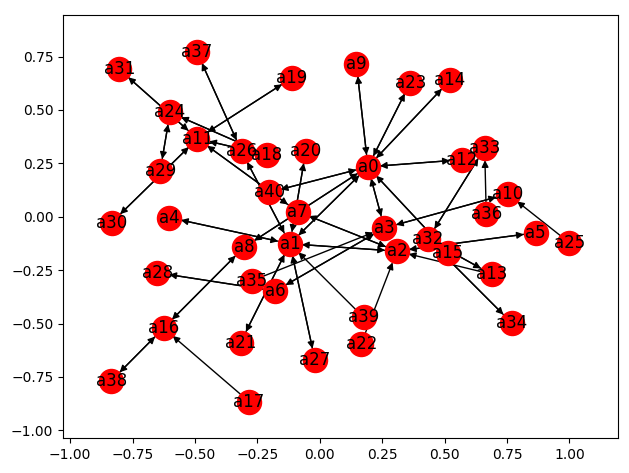
\includegraphics[width=\textwidth]{medium}
	\caption{Medium sized argumentation framework}
	\label{fig:mediumAF}
\end{figure}

In terms of ALIAS Web Extension, the performance and scalability requirements are mostly concerned with the time required to load and render any given Argumentation Framework. User should be able to display and work on large graphs in the UI. On the other hand, the performance of any operation on the given Argumentation Framework will be highly dependent on the performance of ALIAS.

\paragraph{Ease of Use}

Another aspect of non-functional requirements is the ease of use of the application. Original ALIAS application has been implemented in Python, an interpreted, high-level programming language \citep{millman2011python}. Although Python has been designed as the general purpose language, it became very popular. Furthermore, availability of libraries like NumPy and SciPy, it became a popular choice for high-level scientific code development \citep{perez2011python}. Thus, the Python implementation of abstract argumentation semantics solver without the need to setup the environment in any way prior to using it would be beneficial. Being able to install the ALIAS from the PyPi, the Python package manager \citep{pypi}, and use it 'out of the box', gives it an advantage over other solvers.

Ease of use requirement is further addressed by the ALIAS Web Interface. By providing the User Interface, the application is more readily available for anyone wishing to explore and work with Argumentation Frameworks. Web UI removes any need for programming skills as the user would be able to interact with ALIAS through the API.

\paragraph{Design} 
Design functionality is concerned with the User Interface design. The Web Interface should have intuitive and minimalistic design to maximize the space for Argumentation Framework graphs. Available functionality should be easily recognized through descriptive links or buttons.
\subsection{Maximal Conflict Free Sets}
According to the definitions \ref{def:preferredExtension} and \ref{def:stableExtension}, Preferred and Stable extensions are based on the maximal sets. Preferred extensions are the maximal element with respect to the set from all the admissible sets, and Stable extensions are the maximal conflict free sets that attack every argument outside those sets. Furthermore, since each admissible set is also a conflict free set, this property has been used in exploring possible solutions for computing Preferred and Stable extensions.

Let \textit{args} be a collection of arguments in a given argumentation framework \textit{AF}. Then \textit{args} can be represented as $args=arg_1, arg_2,...,arg_n$ where \textit{n} is the total number of arguments in \textit{AF}. 
Furthermore, set of arguments \textit{CF} is conflict free, if and only if there are no attacks between the arguments within the set \textit{CF}: $\forall a,b \in AF, (a, b) \notin attacks$.

Hence, the maximal conflict free sets can be represented as:
\begin{equation}
\begin{array}{lr}
args_1 $ = $ \text{args} $ - $ \text{a} \\
args_2 $ = $ \text{args} $ - $ \text{b} \\
\end{array} \bigg| \forall a, b \in AF, (a,b) \in attacks
\end{equation}

Based on the proposition above, the maximal conflict free set can be calculated by splitting the existing sets of arguments within the given argumentation framework by each pair of arguments from the \textit{attacks}. The process is shown in example in figure \ref{fig:mcfExample}. The Argumentation Framework \textit{AF} consist of four arguments: a, b, c, d, and 3 attacks: a attacks b, b attacks c, and d attacks c. This argumentation framework is presented in figure \ref{fig:af1}. 

\begin{figure}[h]
	\centering
	\includegraphics[width=\linewidth]{"img/mcf "}
	\caption{Maximal Conflict Free sets creation example}
	\label{fig:mcf}
\end{figure}

Firstly, the attack \textit{(a,b)} is applied to the set of all arguments - \textit{\{a,b,c,d\}}, causing the set of arguments to split into two separate sets: one that does not contain argument \textit{b} - \textit{\{a,c,d\}}; and another that does not contain argument \textit{a} - \textit{\{b,c,d\}}. Then each attack from the argumentation framework is applied to the newly created sets, splitting them further into conflict free sets. Attack \textit{(b,c)} has impact only on the second set - \textit{\{b,c,d\}}, since argument \textit{b} is removed from the first set. Hence, applying the second attack to the sets, creates 3 sets: \textit{\{a,c,d\}}, \textit{\{c,d\}} and \textit{\{b,d\}}. Last attack - \textit{(c,d)}, has only impact on the first and second sets from the last step, giving the final set of Maximal Conflict Free sets of \textit{\{a,c\}}, \textit{\{a,d\}} and \textit{\{b,d\}}.

\begin{algorithm}
	\caption{Maximal Conflict Free sets calculation}\label{mcfPseudocode}
	\nl \textit{args} $\gets$ \textit{arguments from AF}\;
	\nl \textit{attacks} $\gets$ \textit{attacks of AF}\;
	\nl \textit{conflictFreeSets} \;
	\nl\ForEach{\textit{attack} $\in$ \textit{attacks}}
	{
		\If{\textit{conflictFreeSets} is not empty}{
				\nl \ForEach{set $\in$ conflictFreeSets}{
					\If{attack[0] $\in$ set AND attack[1] $\in$ set}{
						\nl \textit{conflictFreeSets} += \textit{set} - \textit{\{attack[0]\}} \;
						\nl \textit{conflictFreeSets} += \textit{set} - \textit{\{attack[1]\}} \;
						\nl \textit{conflictFreeSets} -= \textit{set} \;
					}
				}
			}
		\Else{
			\nl \textit{conflictFreeSets} += \textit{args} - \textit{\{attack[0]\}} \;
			\nl \textit{conflictFreeSets} += \textit{args} - \textit{\{attack[1]\}} \;
		}
	}
	\label{alg:mcf}
\end{algorithm}

\subsubsection{Sets}

The algorithm \ref{alg:mcf} is the representation of calculation of the Maximal Conflict Free sets. Depending on the size of the Argumentation Framework and it's complexity this approach will depend on the creation of the large number of combinations of sets. Furthermore, since the size of the collection of the conflict free sets can be $2^n$, where \textit{n} is the total number of arguments within the framework, iterating through this collection for each attack can be time consuming. Hence, to reduce the cost of running the above algorithm, first implementation involved sets data structures. "Set object is an unordered collection of distinct hashable objects" \citep{python_sets}.

To implement the algorithm the conflict free sets were stored as frozenset inside a set. Since the objects within the set are hashed, it provides fast access to its elements. Furthermore, testing membership within the set is performed in the constant time as it does not need to iterate through the whole set as it is the case with list data structure as it can be seen in table \ref{table:timingsMembership}. Additional benefit of using set is its property of being a collection of distinct objects. This helps to ensure that the duplicate sets are not stored, reducing the time required to iterate through the frozensets.

\begin{table}[h]
	\centering
	\caption{Timing in sec for testing membership (10,000 repetitions)}
	\label{table:timingsMembership}
	\begin{tabular}{lllll}
		\hline
		Number of members & 10    & 100   & 1000   & 10000 \\ \hline
		Set                & 0.011 & 0.038 & 0.472  & 4.898 \\
		List               & 0.015 & 0.558 & 54.401 & 57248.254 \\     
	\end{tabular}
\end{table}

Although the set data structure is superior to list in terms of performance, it has a massive overhead in terms of memory usage. Since its objects are hashed it is memory intensive especially for large collections. As can be seen in table \ref{table:sizeDataStructures}, for 10000 elements, the size of the set is over five times of the list. Since the implementation used set of frozensets, the required memory was growing exponentially for bigger argumentation frameworks, making the solution unusable.

\begin{table}[h]	
	\centering
	\caption{Size of data structures in bytes}
	\label{table:sizeDataStructures}
	\begin{tabular}{lllll}
		\hline
		Number of elements & 10  & 100  & 1000  & 10000  \\ \hline
		Set                & 736 & 8416 & 32992 & 524512 \\
		List               & 200 & 1008 & 9112  & 90112 
	\end{tabular}
\end{table}

% add some results from alias

\subsubsection{PyTable}
In order to try resolve the memory issue caused by the large set of frozensets, attempt has been made to implement the solution for Maximal Conflict Free sets using PyTables. PyTables is a python module for "managing hierarchical datasets and designed to efficiently and easily cope with extremely large amounts of data" \citep{pytables}. It is using HDF5, which is a "data model, library and file format for storing and managing data" \citep{hdf5}. 

Using PyTables for storage of all generated sets will release the huge amount of memory required for using sets of sets. The algorithm used with PyTables is slightly modified version of the algorithm \ref{alg:mcf}. In order to maximize the performance while using PyTables, three tables are created:
\begin{enumerate}
	\item{Arguments Table - table for storing all arguments within the argumentation framework. The table consist of the name of the argument and its mapping}
	\item{Conflict Free Table - table for storing references to conflict free sets. This table consists of only one column - id}
	\item{Argument Conflict Free Bridge Table - this table is used for storing references of arguments within the conflict free sets. Consisting of three columns: argument id, conflict free set id and active flag, links the tables above.}
\end{enumerate}


\subsubsection{Dictionaries}
Another approach to implement the maximal conflict free set algorithm is to use data structure 'defaultdict'. 'Defaultdict' class provides a new dictionary-like object, where the first argument in the constructor specifies default factory attribute. It is a subclass of a standard 'dict' class in Python and majority of the methods are the same between 'defaultdict' and 'dict' classes \citep{defaultdict}.

The implementation uses two 'defaultdict' classes with sets as its default factory attribute. One of the dictionaries is used to store all the arguments from the argumentation framework as the keys and a set of references to the conflict free sets as a value. Second dictionary is used to store the conflict free sets, where the key is just the identifier that gets incremented with every new record and the value is a set of the argument names in that particular conflict free set. Table \ref{table:dictsRepresentation} shows an example of the dictionaries being used to compute the maximal conflict free sets based on the argumentation framework \ref{fig:argumentationFrameworkFigure} from section \ref{abstractArgumentation}.

\begin{table}[h]
	\centering
	\caption{Representation of two dictionaries and their relations for Maximal Conflict Free sets generation}
	\label{table:dictsRepresentation}
	\begin{tabular}{lllll}
		\multicolumn{2}{l}{Arguments}                            &                       & \multicolumn{2}{l}{Conflict Free Sets}                  \\ \cline{1-2} \cline{4-5} 
		\multicolumn{1}{|l|}{Key} & \multicolumn{1}{l|}{Value}   & \multicolumn{1}{l|}{} & \multicolumn{1}{l|}{Key} & \multicolumn{1}{l|}{Value}   \\ \cline{1-2} \cline{4-5} 
		\multicolumn{1}{|l|}{a}   & \multicolumn{1}{l|}{\{1,2\}} & \multicolumn{1}{l|}{} & \multicolumn{1}{l|}{1}   & \multicolumn{1}{l|}{\{a\}}   \\ \cline{1-2} \cline{4-5} 
		\multicolumn{1}{|l|}{b}   & \multicolumn{1}{l|}{\{3,4\}} & \multicolumn{1}{l|}{} & \multicolumn{1}{l|}{2}   & \multicolumn{1}{l|}{\{a,c\}} \\ \cline{1-2} \cline{4-5} 
		\multicolumn{1}{|l|}{c}   & \multicolumn{1}{l|}{\{2\}}   & \multicolumn{1}{l|}{} & \multicolumn{1}{l|}{3}   & \multicolumn{1}{l|}{\{b\}}   \\ \cline{1-2} \cline{4-5} 
		\multicolumn{1}{|l|}{d}   & \multicolumn{1}{l|}{\{4\}}   & \multicolumn{1}{l|}{} & \multicolumn{1}{l|}{4}   & \multicolumn{1}{l|}{\{b,d\}} \\ \cline{1-2} \cline{4-5} 
	\end{tabular}
\end{table}

As can be seen in table \ref{table:dictsRepresentation}, there is a direct link between the arguments and conflict free sets dictionaries. The benefit of using a dictionaries as a data structure is that the retrieval of keys are a very fast operation, as those are usually implemented as a hash tables \citep{pythonDictionary}. Hence, the implementation is operating on two dictionaries simultaneously in order to provide the quick retrieval of the values based on the keys, while keeping the memory usage at a low level compared to using sets of sets.

% comparison of memory usage of defaultdict

There are number of steps that need to be taken in order to compute the maximal conflict free set using the dictionaries. Firstly, the sets to be modified need to be found, based on the attack tuple being added - this is simply intersection of the sets from arguments dictionary for the attacking and attacked argument. Then for all the values from that intersection, access the sets in conflict free sets dictionary and replace the existing set with two copies of that set: one without the attacker and one without the attacking arguments. The final step is to update the arguments dictionary by updating the references to the conflict free sets for all the arguments that were included in that set.

% some performance chart?

The operations in the approach above consists of accessing the values from the dictionary and performing simple operations on sets. Those operations are performed relatively quickly. However, similarly to other approaches, the number of sets in the conflict free sets dictionary in the worst case scenario will exponentially grow with each attack being added. If the argumentation framework is linear, i.e. a attacks b, b attacks c, c attacks d, etc., then with each attack that is processed the number of conflict free sets and number of operations will double, ultimately giving $O(n^2)$ big O notation in the worst case scenario. 




\subsection{Boolean Satisfiability Solver} \label{section:satSolver}
In order to improve the performance and based on the results of analysis of existing solvers an attempt has been made to reduce the problem into boolean satisfiability problem. 

\subsubsection{PicoSAT and PycoSAT} \label{section:pycosat}
PicoSAT is a Boolean Satisfiability Solver for boolean variables in boolean expressions written by Armin Bierre \citep{picosatMan}. Implemented in C and optimized with compact data structures for watching literals provides a high performance solver capabilities with low memory usage \citep{picosat}.

PycoSAT is a Python package that provides direct translation for interacting with PicoSAT \citep{pycoSat}. The advantage of PycoSAT is that it imports the PicoSAT binaries directly, which removes the hassle of manually building the solver. PycoSAT provides only two functions \citep{pycosatPyPi}: 
\begin{enumerate}
	\item \textit{solve} - where only a single solution is returned, or the "UNSAT" string when the clauses are unsatisfiable
	\item \textit{itersolve} - returns iterator over solutions
\end{enumerate}

The advantage of PycoSAT is the ability to easily create clauses in form of boolean conjunctions of disjunctions. Hence, encoding the conflict-free, admissible sets and extensions can be easily achieved. PycoSAT clauses are defined in terms of list of lists. In order to show the encodings let consider the example from PycoSAT documentation \citep{pycosatGithub}. 

\begin{figure}
\begin{tcolorbox}
	p cnf 5 3 \\
	1 -5 4 0 \\ 
	-1 5 3 4 0 \\
	-3 -4 0 
\end{tcolorbox}
\caption{Example of PycoSAT problem}
\label{fig:pycosat1}
\end{figure}

The above example represents the example clauses encoded using DIMACS CNF format. The first line of the example is used to provide information about the clauses. \textit{p} stands for \textit{problem} and indicates that this line is used to define the problem to be solved. \textit{cnf} describes the file type, which is followed by the number of variables and clauses. Hence, we can conclude that this particular problem contains 5 variables and 3 clauses. 

The following 3 lines are representing individual clauses. Each number represents one of the 5 variables and the sign next to the number shows whether the variable should or should not be included in the solution. Hence, the first line can be translated into $ a_1 \lor \neg a_5 \lor a_4 \lor a_0 $. 

\begin{figure}
\begin{minted}{python}
	>>> import pycosat
	>>>
	>>> cnf = [[1, -5, 4], [-1, 5, 3, 4], [-3, -4]]
	>>> for sol in pycosat.itersolve(cnf):
	...	    print(sol)
\end{minted}
\caption{PycoSAT usage example}
\label{fig:pycosatUsage}
\end{figure}

Example from figure \ref{fig:pycosat1} can be translated into list of lists and used with PycoSAT as shown in figure \ref{fig:pycosatUsage}. The clauses encodings are passed into itersolve method of PycoSAT, which in turn returns iterator. The example above will produce following output:

\begin{figure}
	\begin{minted}{python}
[1, -2, -3, -4, 5]
[1, -2, -3, 4, -5]
[1, -2, -3, 4, 5]
[1, -2, 3, -4, -5]
[1, -2, 3, -4, 5]
[1, 2, 3, -4, -5]
[1, 2, 3, -4, 5]
[1, 2, -3, -4, 5]
[1, 2, -3, 4, -5]
[1, 2, -3, 4, 5]
[-1, 2, -3, 4, -5]
[-1, 2, -3, 4, 5]
[-1, 2, -3, -4, -5]
[-1, 2, 3, -4, -5]
[-1, -2, 3, -4, -5]
[-1, -2, -3, -4, -5]
[-1, -2, -3, 4, 5]
[-1, -2, -3, 4, -5]
	\end{minted}
	\caption{PycoSAT example output}
	\label{fig:pycosatOutput}
\end{figure}

The output presented in figure \ref{fig:pycosatOutput}, is the list of all possible combination of 5 variables that satisfy the clauses from figure \ref{fig:pycosat1}. With appropriate mapping, the values from output can easily be replaced with variables to create individual solutions. 



\subsubsection{CNF Encodings}
In order to use any SAT solver to solve the extensions of argumentation frameworks, the boolean formula needs to be encoded into CNF. The conflict free sets can easily be encoded using the list of all the attacks in the argumentation framework. From the definition of the conflict free sets we know that it is a set of arguments with no attacks between any of its elements. Hence, for each attack in the argumentation framework, the conflict free set will contain either the attacker, or the attack. In no case both of the arguments will be a part of the same conflict free set. This can be shown in CNF as:

\begin{equation}
	  \forall (a,b) \in attacks \implies (\neg a \lor \neg b)
\end{equation}

The above equation will provide all of the possible solution based on the arguments provided for the conflict free sets. This can be extended further to include the defending arguments of the set. This in turn will help to define the admissible sets, as based on the definition \ref{admissibleArgument}, the admissible set contains conflict free arguments and all arguments within the set that are defended by the set itself.

\begin{equation}
\forall a \in AF | (a,b) \in attacks \land \exists c \in E | (c,a) \in attacks \implies (c \lor \neg b)
\end{equation}

In the equation above, we see that for the set \textit{E} to be admissible there must be argument \textit{a} that attacks \textit{b}, and some argument \textit{c} in set \textit{E}, such that \textit{c} attacks \textit{b}. This definition can be encoded in boolean form as \textit{c} or \textit{not b}. Hence, if the argument \textit{b} is included in the model, then argument \textit{c} is ignored, as the clause will evaluate to \textit{true} based on the $\neg b$ being itself \textit{true}. However, if argument \textit{b} is included in the model, then argument \textit{c} will have to be included in the same model in order for the clause to evaluate to \textit{true}.
\section{Extensions}
ALIAS has been implemented to provide all admissible sets from the SAT solver. Those sets are then verified if they are part of the requested extension. 


\subsection{Stable Extension} \label{section:stableExtension}
Based on the definition \ref{def:stableExtension}, Stable Extension is the conflict-free set that attacks all arguments not included in the set. This makes verifying the Stable Extension a straightforward process using just a set theory: attacks of the set to be verified has to be equal to the set of arguments not included in the set to be checked. If those are equal, then the set in question is a stable extension, since there are no other arguments that are neither attacked by this set nor included in it. Hence, ALIAS verifies all the solutions provided by the SAT solver using the above property of the extension. This can be represented as: 

\begin{equation}
R^+(S) = args \oplus S
\end{equation}

where $S$ is the set of arguments to be verified, $R^+(S)$ represents the arguments attacked by the set $S$, and $\oplus$ indicates the symmetric difference. If the above equation evaluates to \textit{true}, the set being checked is added to the list of extensions, otherwise, it is ignored. Once all the sets have been checked, the generated list is returned.

\subsection{Matrices}
Matrix in mathematics is an 2 dimensional array with predefined number \textit{n} of rows and \textit{m} of columns: \textit{n x m} matrix \citep{matrices}, where each individual cell within the matrix stores information. Matrix with equal number of rows and columns is called a square matrix. 

As it was shown in the definition \ref{AFdef}, abstract argumentation is a collection of finite arguments and relations between those arguments. Hence, argumentation frameworks can be easily represented in the form of matrices, where both rows and columns represent the arguments within the framework and their relations are marked in each individual cells. 

If we consider the argumentation framework from figure \ref{fig:argumentationFrameworkFigure}, it can be seen that it consists of four arguments: a, b, c and d. Furthermore, it can be observed that a is attacking b, b is attacking c and c is also attacked by d. Hence, the argumentation framework can be represented as a 4 x 4 matrix shown in figure \ref{fig:matrixRepresentation}.

\begin{figure}[h]
\centering
	\begin{blockarray}{ccccc}
		  & a & b & c & d\\
		\begin{block}{c[cccc]}
			a & 0 & 1 & 0 & 0 \\
			b & 0 & 0 & 1 & 0 \\
			c & 0 & 0 & 0 & 0 \\
			d & 0 & 0 & 1 & 0 \\
		\end{block}	
	\end{blockarray}
	\label{fig:matrixRepresentation}
	\caption{Matrix representation of Argumentation Framework from figure \ref{fig:argumentationFrameworkFigure}}
\end{figure}

The only values used within the matrix are 0 and 1, where 1 indicates that there is a relation between the arguments from the relevant row and column. Furthermore, the direction of the attack can be easily described in the matrix, where each row represents a single argument, and the columns are used to show any relations to other arguments directed from that particular argument. Hence, when argument \textit{a} attacks argument \textit{b}, cell $M_{ab}$ has value 1, as shown in figure \ref{fig:matrixRepresentation}. In case the argument is a self attacking, the matrix value for a cell \textit{i, j}, where \textit{i} = \textit{j}, would be set to 1 \citep{afmatrices1}.

As \citet{afmatrices1} points out, matrices can only be used to answer a single question with reasonable efficiency from the work of \citet{bench2007argumentation}: 'Is \textit{A} an extension?'. And although \citet{afmatrices1} implemented a system called ASSA \citep{assa}, to compute all stable extensions using purely matrices, this approach is inefficient. In order to find all stable extensions the proposed solver needs to convert all possible instances of the selected set of arguments into a vector form. It then combines all vectors into a single massive matrix \citep{afmatrices1}. Thus, the proposed approach is ineffective, especially when compared to other available solvers.

\citet{matrix2} in their paper presented a different approach of using the matrices to verify if the given set is an extension. The argumentation framework can be divided into three parts: 
\begin{enumerate}
	\item The conflict-free set $S$
	\item The attacked set: $R^+(S)$
	\item The remaining set: $A\setminus (S\cup R^+(S))$
\end{enumerate}

By using sub-blocks of the matrix for different parts of the argumentation framework and transforming the matrix into one of the two standard forms, the proposed approach allows checking if the given set is conflict-free, admissible, stable, complete, preferred and grounded extensions \citep{matrix2}.

This approach has been used in ALIAS to verify complete and preferred extensions.

\subsection{Complete Extension}
The implementation for verifying if the given set is a Complete Extension is based on the approach presented by \citet{matrix2}. By dividing the matrix into certain sub-blocks, they found a dependency between column and row vectors that allow confirming if the set is, in fact, a complete extension.

Lets consider an example presented by \citet{matrix2}: given the argumentation framework $AF = (Args, attacks)$, where $Args = \{1,2,3,4,5\}$ and $attacks = \{(2,5), (3,4), (4,3), (5,1), (5,3)\}$, it can be represented in a graph as shown in figure \ref{fig:exampleAF}.

\begin{figure}[h]
	\tikzset{
		main/.style={draw, rectangle, rounded corners, minimum height=1cm, minimum width=4.5cm},
		arrow/.style={thick,<-,>=stealth}
	}
	\centering
	\begin{tikzpicture}[auto,node distance=1.5cm]
	\coordinate(coor);
	\node[draw=none,fill=none][above=0.75cm of coor](2){2};
	\node[draw=none,fill=none][below=0.75cm of coor](1){1};
	\node[draw=none,fill=none][right=of coor](5){5};
	\node[draw=none,fill=none][right=of 5](3){3};
	\node[draw=none,fill=none][right=of 3](4){4};			
	%%% ARROWS %%%
	\draw[arrow](5) -- (2);
	\draw[arrow](1) -- (5);
	\draw[arrow](3) -- (5);
	\draw[thick,<-,>=stealth,transform canvas={yshift=-0.2em}](3) -- (4);
	\draw[thick,<-,>=stealth,transform canvas={yshift=0.5em}](4) -- (3);
	\end{tikzpicture}
	\caption{Argumentation Framework \ref{fig:exampleAF}}
	\label{fig:exampleAF}
\end{figure}

The above argumentation framework can also be represented in form of the matrix as shown in figure \ref{fig:exampleAFMatrix}.

\begin{figure}[h]
	\centering
	\begin{blockarray}{cccccc}
		& 1 & 2 & 3 & 4 & 5\\
		\begin{block}{c[ccccc]}
			1 & 0 & 0 & 0 & 0 & 0 \\
			2 & 0 & 0 & 0 & 0 & 1 \\
			3 & 0 & 0 & 0 & 1 & 0 \\
			4 & 0 & 0 & 1 & 0 & 0 \\
			5 & 1 & 0 & 1 & 0 & 0 \\
		\end{block}	
	\end{blockarray}
	\caption{Matrix representation of Argumentation Framework from figure \ref{fig:exampleAF}}
	\label{fig:exampleAFMatrix}
\end{figure}

Lets consider an admissible set $S = \{1,2\}$. In order to verify if the set $S$ is complete, the matrix should be divided into sub-blocks as shown in figure \ref{fig:subblocks}. The green area represents the set $S = \{1,2\}$, orange sub-block relation between the set $S$ and the remaining arguments indicated by $M^s(\{1,2\})$, while yellow sub-block of arguments not included in the set $S$ indicated by $M^c(\{1,2\})$. 

\citet{matrix2} propose the following theorem:
\begin{theorem}
Given $AF = (A, R)$ with $A = {1, 2, ..., n}$, an admissible extension $S = {i_1, i_2, ..., i_k} \subseteq A$ is complete if and only if:
\begin{enumerate}\label{theorem:completeMatrix}
	\item some column vector $M^s_{*,p}$ of the s-sub-block $M^s(S)$ is zero, then its corresponding column vector $M^c_{*,p}$ of the c-sub-block $M^c(S)$ is non-zero, and
	\item for each non-zero column vector $M^c_{*,p}$ of the c-sub-block $M^c(S)$ appearing in (1), there is at least one non-zero element $a_{j_q,j_p}$ of $M^c_{*,p}$ such that the corresponding column vector $M^s_{*,q}$ of the s-sub-block $M^s(S)$ is zero, where $\{j_1,j_2,...,j_h\} = A\backslash S$ and $1\leq q,p \leq h$.
\end{enumerate}
\end{theorem}


\begin{figure}[h]
	\centering
	\begin{tabular}{llllll}
		& \textbf{1} & \textbf{2} & \textbf{3} & \textbf{4} & \textbf{5} \\ \hline
		\multicolumn{1}{l|}{\textbf{1}} & \cellcolor[HTML]{32CB00}{\color[HTML]{FFFFFF} \textbf{0}} & \cellcolor[HTML]{32CB00}{\color[HTML]{FFFFFF} \textbf{0}} & \cellcolor[HTML]{F8A102}\textbf{0} & \cellcolor[HTML]{F8A102}\textbf{0} & \cellcolor[HTML]{F8A102}\textbf{0} \\
		\multicolumn{1}{l|}{\textbf{2}} & \cellcolor[HTML]{32CB00}{\color[HTML]{FFFFFF} \textbf{0}} & \cellcolor[HTML]{32CB00}{\color[HTML]{FFFFFF} \textbf{0}} & \cellcolor[HTML]{F8A102}\textbf{0} & \cellcolor[HTML]{F8A102}\textbf{0} & \cellcolor[HTML]{F8A102}\textbf{1} \\
		\multicolumn{1}{l|}{\textbf{3}} & 0 & 0 & \cellcolor[HTML]{FCFF2F}{\color[HTML]{000000} \textbf{0}} & \cellcolor[HTML]{FCFF2F}{\color[HTML]{000000} \textbf{1}} & \cellcolor[HTML]{FCFF2F}{\color[HTML]{000000} \textbf{0}} \\
		\multicolumn{1}{l|}{\textbf{4}} & 0 & 0 & \cellcolor[HTML]{FCFF2F}{\color[HTML]{000000} \textbf{1}} & \cellcolor[HTML]{FCFF2F}{\color[HTML]{000000} \textbf{0}} & \cellcolor[HTML]{FCFF2F}{\color[HTML]{000000} \textbf{0}} \\
		\multicolumn{1}{l|}{\textbf{5}} & 1 & 0 & \cellcolor[HTML]{FCFF2F}{\color[HTML]{000000} \textbf{1}} & \cellcolor[HTML]{FCFF2F}{\color[HTML]{000000} \textbf{0}} & \cellcolor[HTML]{FCFF2F}{\color[HTML]{000000} \textbf{0}}
	\end{tabular}
	\caption{Matrix sub-blocks of Argumentation Framework \ref{fig:exampleAF} for set $S = \{1,2)\}$}
	\label{fig:subblocks}
\end{figure}

From the figure \ref{fig:subblocks}, it can be seen that the $M^s(\{1,2\})$, contains two zero column vectors: $M^s_{*,1} = \begin{pmatrix}
0\\ 
0
\end{pmatrix}$ and $M^s_{*,2} = \begin{pmatrix}
0\\ 
0
\end{pmatrix}$ . Their corresponding column vectors in $M^c(\{1,2\})$ are $M^c_{*,1} = \begin{pmatrix}
0\\ 
1\\ 
1
\end{pmatrix}$ and $M^c_{*,2} = \begin{pmatrix}
1\\ 
0\\ 
0
\end{pmatrix}$, which are all non-zero. Furthermore, for $a_{43} = 1$ in $M^c_{*,1}$, the corresponding column vector $M^s_{*,2}$ in $M^s(\{1,2\})$ is zero. And for $a_{34} = 1$ in $M^c(\{1,2\})$, the corresponding column vector $M^s_{*,1}$ in $M^s(\{1,2\})$ is also zero. Hence based on the theorem \ref{theorem:completeMatrix}, subset $S = \{1,2\}$ is a Complete Extension of $AF$.

In order to implement this in Python, SciPy \citep{jones2014scipy} sparse matrix object has been used. Class Matrix has been created that takes the responsibility of matrix creation and accessing the required sub-blocks of the matrix. Once the solver provides a possible solution, then both C and S sub-blocks of the matrix are fetched. Once all the required data is gathered, the first condition of the theorem \ref{theorem:completeMatrix} can be verified. The columns of each sub-block are summed, zipped together and compared. If the sum of the corresponding columns in s-block and c-block are equal to 0 then the application breaks out of the method returning False. 

Once all the column sums have been checked the application can move to the second condition of the theorem. Search is performed to filter out all the elements from c sub-block with value 1. For each element $a_{i,j}$ from the generated list, the corresponding value from the sum of columns of s sub-block is checked. The dictionary holding results for all columns is updated setting the value to either True if the corresponding column vector from s sub-block is 0, or False otherwise. There are additional checks to ensure the record does not already exist in the dictionary, as this condition has to be met for at least one non-zero element from each column vector of c sub-block.

After checking all elements from C and S sub-blocks, the dictionary storing results of the second conditions is checked. If any of the elements of the dictionary is set to false, the method returns false and the set is not considered as part of the complete extension. 

\subsection{Preferred Extension} \label{section:preferredExtension}
Preferred extensions are checked in a similar way to the Complete Extensions above. By definition \ref{def:preferredExtension}, Preferred Extension is the maximal, with respect to set inclusion, an admissible set of arguments. Hence, the only checks we have to do is to verify if the given set is admissible and if it is maximal with respect to set inclusion.

Similarly to the complete extension, SciPy matrix representations have been used for the argumentation frameworks. Once the solver generates a possible solution, the fetch of arguments to be checked is performed. However, in the case of the Preferred extension, the application only fetches the arguments not included in the proposed solution and not attacked by the solution. Hence, the required matrix is a c sub-block without the attacked set $R^+(S)$.
 
Once the solver fetches required sub-block it sums all the column vertices. This creates a single list of sums for all arguments not being attacked by the set $S$. Finally, the algorithm iterates through that list to check if any value is equal to 0. If it is, then the set of arguments being currently checked is not a preferred extension. Otherwise, the method will return the true and that set of arguments will be added to the list of preferred extensions.

\section{Testing} \label{section:testing}
ALIAS was being developed using iterative approach. For each iteration a different approach for computing the extensions has been implemented. In order to verify and benchmark the approach, each iteration had allocated time for testing. Furthermore, the testing process can be divided into two separate processes: 
\begin{enumerate}
	\item Unit testing - number of tests created to verify the correctness of the proposed solution. Those tests are to verify if any change to the solution still produces correct output. 
	\item Benchmark testing - more extensive testing carried out at the end of each iteration. The purpose of the benchmark testing is to help evaluate the system. 
\end{enumerate}


As described in section \ref{label:projectRequirements}, there are number of functional and non-functional requirements for ALIAS. One of the most critical set of requirements identified are the correctness of computed solution and the scalability. In order to verify those requirements the black-box testing technique was used. Black box testing as described by \citet{testing2} is "based on the analysis of the specification of a piece of software without reference to its internal working". Hence, during the benchmark testing, the results were based on the output of the system and its response time. With no regards to the inner workings of the application, it allows examine only the fundamental workings of the system. Thus, in order to use the black-box testing, the final testing for each approach was done once the implementation was finished \citep{blackbox}.

In order to extensively test ALIAS, benchmark argumentation frameworks have been taken from the published sample argumentation frameworks from ICCMA 2017 \citep{iccmaResults}. The website provides 5 different sets of argumentation frameworks for all tasks involved in the competition and additional set for a Dung's Triathlon. Selected argumentation frameworks have been classified into 5 categories: very easy, easy, medium, hard and too hard. Appendix \ref{appendix:benchmarkFiles} shows the full list of argumentation frameworks used including the number of arguments and attacks. Although, different set of frameworks have been used for testing preferred and complete, and stable extensions, it can be seen that the sizes and complexity of the argumentation frameworks used differ. Starting from small framework including only 2 arguments and single attack the complexity increases to as much as six thousand arguments and over sixty thousand attacks in some cases. This is to help identify limits and possible issues with proposed solution. 

Additional benefit of using the benchmark frameworks from ICCMA 2017 competition is to be able to compare the results of ALIAS against the existing solutions. Furthermore, the benchmark testing can help identify the best solution and aid with improving the approach used. With satisfactory results, ALIAS could take a part in the future competitions.

\subsection{Unit testing}
Unit tests played important role during the development of each approach for ALIAS. Every change to the proposed solution has been tested and verified by using small number of argumentation frameworks. Each framework has been created and tested using other systems like Pyglaf and ArgSemSAT to ensure the outputted extensions are correct. 

Although unit testing does not help with evaluating the overall performance of ALIAS it played critical role during the development of the system. 

\subsection{Performance}
As \citet{performanceTesting1} points out the performance requirements play a key role in determining the usability and quality of many systems. In case of ALIAS the biggest concern in terms of performance is scalability. Argumentation frameworks used for unit testing were small in comparison to frameworks used in real world application or competitions like ICCMA. Thus, to correctly evaluate the performance and abilities of ALIAS, the benchmark argumentation frameworks have been used.

In order to test the scalability and performance, each implemented solution has been put through extensive testing. For each extension implemented within the proposed solutions, tests have been executed using the appropriate argumentation frameworks from appendix \ref{appendix:benchmarkFiles}. Each test run has been executed on the same machine with following specifications:

\begin{itemize}
	\item Processor: Intel Core I5-6200U @ 2.30 GHz
	\item GPU: Nvidia GeForce 940MX
	\item RAM: 8GB
	\item OS: Linux based
\end{itemize}

Using the same specifications for each test run allows for the test results to be easily comparable. Furthermore, since ICCMA 2017 competition has been ran on a different machines, Pyglaf \citep{pyglaf} and ArgMatSAT \citep{argmatSat} have been put through the same benchmark testing. Those results were used to compare and evaluate the performance of ALIAS to the most successful solvers submitted to ICCMA 2017.

During the testing, the CPU time has been limited per each argumentation framework to 20 minutes. This is to prevent the solver from computing the extensions indefinitely, especially on larger and more complex argumentation frameworks. The time required to read and parse files was not included in the specified time limit and it was used purely for computing all extensions. 

There were four separate proposed solution for computing abstract argumentation. Three of them were using the same method of computing the maximal conflict free set, but using different data structures to overcome certain issues and limitations as described in section \ref{section:maxConflictFreeSet}. The final approach is using SAT solver to enumerate possible solutions (see section \ref{section:satSolver}). Each approach was generating a number of possible solutions, which were then verified using matrix approach for preferred extension and set inclusion for stable extension as shown in sections \ref{section:preferredExtension} and \ref{section:stableExtension} respectively. 

\subsubsection{Stable Extension results}

\begin{figure}[h]
	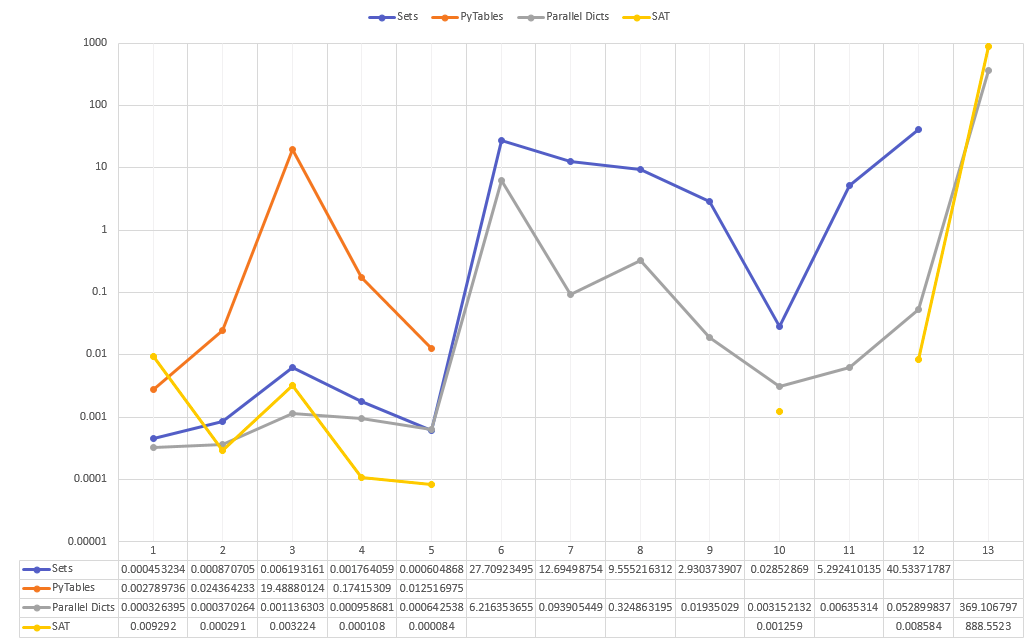
\includegraphics[width=\textwidth]{stable_results}
	\caption{Timings of 4 approaches computing Stable Extension}
	\label{fig:stableFinalResults}
\end{figure}

Figure \ref{fig:stableFinalResults} shows the execution times of all four approaches: sets, PyTables, parallel dictionaries and SAT solver for computing all Stable Extension on the set of argumentation frameworks specified in appendix \ref{appendix:benchmarkFiles}. The chart only shows the timings for the first 13 frameworks. Almost most of the approaches failed to produce the results for the remaining frameworks within the specified 20 minutes time limit. Furthermore, as can be seen in the chart \ref{fig:stableFinalResults}, certain data points are missing for some of the approaches. This is also due to the solver reaching a 20 minutes time limit without providing the solution. 

As can be seen in figure \ref{fig:stableFinalResults}, only approach using parallel dictionaries managed to compute the stable extensions for those frameworks in the specified time. Furthermore, it has the shortest execution time for majority of the frameworks across all approaches, with exception for five of them, where SAT solver approach considerably outperformed it. The execution time of dictionaries approach closely correspond to the approach using sets. Although sets operation are highly optimized in Python, it still did not outperform the implementation using dictionaries.

The worst performing solution is the PyTables approach to computing and storing the Maximal Conflict Free Sets. This approach only computed the extensions for first five argumentation frameworks provided, which had the lowest number of arguments and relations between them. Those results are due to dynamically creating the sets iterating through all the attacks within the argumentation framework as shown in section \ref{section:maxConflictFreeSet}. Since PyTables stores data on the hard drive, the read/write access creates high latency in terms of getting and storing values. This in turn has impact on the overall performance of the solution. 

Although the sets and dictionaries approaches for Maximal Conflict Free Sets creation produced results for most of the provided argumentation frameworks, they have a massive overhead - memory usage. The tests were performed on the machine with 8GB RAM available for the solver and another 8GB swap memory. Both of the solutions: sets and dictionaries, were running out of memory space for any framework with 20 or more arguments. Since this approach is combinatorial and generates all the possible maximal conflict free sets first, the number of combinations is extremely high. Hence, storing all possible sets is memory expensive as in the worst case scenario it will generate $2^n$ records, where $n$ is the number of arguments in the framework.

SAT based approach tends to outperform other solutions for frameworks it managed to complete the computation. As can be seen in figure \ref{fig:stableFinalResults}, half of the timings for SAT solver approach are considerably faster than other approaches. Only in 3 instances, this approach was slower than approach using dictionaries. However, as shown in the section \ref{section:satSolver}, SAT based approach uses a simple encodings for the admissible sets. Due to the size of argumentation frameworks used for testing, it caused the solver to reach the 20 minutes time out for 5 of the frameworks used for comparison. 

\subsubsection{Preferred Extension results}

\subsection{Correctness}
Correctness of the computed semantic is the critical functionality of the successful solver. However, this introduce the challenge of finding the best way to verify the produced solution. There are number of formal approaches that could be applied to the solver in order to confirm it provides the correct answer. For example, formal method called Z, "formal specification methodology that can dramatically improve the way software systems are modeled and implemented" \citep{potter1996introduction}, could be used to model the application and provide the proof of correctness. Although defining the approach and modeling the system could provide the guarantee for the correctness of the application, this is outside of the scope of this project. 

Thus, In order to test and verify the correctness of ALIAS, the same argumentation frameworks from appendix \ref{appendix:benchmarkFiles} have been used as for the performance testing. The outputs of the SAT based approach have been compared to the results of two winning solvers: Pyglaf \citep{pyglaf} and ArgSem-SAT \citep{argsemsat}. Although this does not guarantee the correct results, those solvers were the two highest scoring solvers in the competition and if their results are equal, the probability of answer being incorrect is low.

\subsection{Web UI Test Cases}


\section{Evaluation} \label{section:evaluation}

-------------------------------------------------------------------------------\\
\textbf{Points to discuss}
\begin{enumerate}
	\item{Define clear way of evaluating the project}
	\item{Describe benchmark testing}
	\item{Define analysis of benchmark testing results}
\end{enumerate}
-------------------------------------------------------------------------------\\

The project will be evaluated based on the benchmark testing. Benchmark tests will be performed after each developement cycle and will be used to evaluate the performance and correctness of the software based on the results from the solvers submitted for the second edition of International Competition on Computational Models of Argumentation (http://argumentationcompetition.org/). 
The benchamrk tests will include computing semantics from provided argumentation frameworks. It will be split into 7 tracks. Each track will represent different semantic. Following semantics will be used for benchmark testing:
\begin{enumerate}
	\item{Complete Semantics - CO}
	\item{Preferred Semantics - PR}
	\item{Stable Semantics - ST}
	\item{Semi-Stable Semantics - SST}
	\item{Stage Semantics - STG}
	\item{Grounded Semantics - GR}
	\item{Ideal Semantics - ID}
\end{enumerate}

For each track the system will need to solve following reasoning problems, with the exception for Grounded and Ideal semantics where only A and C are applicable:
\begin{enumerate}
	\item{Given an abstract argumentation framework, determine some extension\\SE-$\sigma$: Given F=(A,R) return some set E $\subseteq$ A that is a $\sigma$-extension}
	\item{Given an abstract argumentation framweork, determine all extensions\\EE-$\sigma$: Given F=(A,R) enumerate all sets E $\subseteq$ A that are $\sigma$-extensions}
	\item{Given an abstract argumentation framework and some argument, decide whether the given argument is credulously inferred\\DC-$\sigma$ : Given F=(A,R), a $\in$ A decide whether a is credulously accepted under $\sigma$}
	\item{Given an abstract argumentation framework and some argument, decide whether the given argument is skeptically inferred\\DS-$\sigma$: Given F=(A,R), a $\in$ A decide whether a is skeptically accepted under $\sigma$}
\end{enumerate}

There are 4 different benchmarks that will be used (all of them were used for testing solvers submitted to ICCMA 2017). Each benchmark group consist of a number of abstract argumentation frameworks in formats \textit{apx} and \textit{tgf}. Furthermore, each group of argumentation frameworks are used for a specific tasks. The list of relations between benchmarks and the tasks is below:
\begin{itemize}
	\item{Benchmark A - DS-PR, EE-PR, EE-CO, DS-SST, DC-SST, SE-SST, EE-SST, DS-STG, DC-STG, SE-STG, EE-STG}
	\item{Benchmark B - DS-ST, DC-ST, SE-ST, EE-ST, DC-PR, SE-PR, DC-CO}
	\item{Benchmark C - DS-CO, SE-CO, DC-GR, SE-GR}
	\item{Benchmark D - DC-ID, SE-ID}
\end{itemize}

Prior to running the benchmarking tests following solvers will need to be tested with the available benchmarks to evaluate their performance in the given environment.
\begin{enumerate}
	\item{pyglaf - CO, ST, ID tracks}
	\item{ArgSemSAT - PR track}
	\item{argmat-sat - SST, STG tracks}
	\item{CoQuiAAS v2.0 - GR track}
\end{enumerate}
Those are the winning solvers in the specified tracks. Once the baseline for benchmark testing will be created, the software testing can commence.

\section{Future Work} \label{section:futureWork}
\section{Overview}
In this section ALIAS solver will be evaluated in terms of functional and non-functional requirements discussed in section 4.2. Each implemented approach will be reviewed in terms of performance. Furthermore, ALIAS will be compared to other solvers in relation to its performance and scalability. Finally, the ease of use will be evaluated.

Another evaluation will be performed on ALIAS web interface. This extension will be evaluated in terms of functionality and usability. 
\section{Functionality}
Not all of the requirements identified in the design stage were implemented in this project. Hence, any functionality not included should be considered as future work. Those include computing additional semantics, such as ground, ideal, semi-stable. Furthermore, ALIAS could be extended to give user possibility of removing arguments and attacks. 

\section{Solver}
ALIAS is using PicoSAT solver with PycoSAT python module as the translation between Python and PicoSAT. As discussed in section \ref{section:pycosat}, PicoSAT is a high-performance solver, which helps to increase the performance of ALIAS itself. However, it has certain limitations. The most noticeable one is the limited ability to encode the clauses. PycoSAT only allows the clauses to be encoded in the format of conjunctions of disjunctions. This can have a big impact on the way semantics are being encoded. Future work might include investigation of alternative solvers with Python interfaces and incorporating them in ALIAS. One of the most noticeable alternatives is a Satisfiability Modulo Theories solver from Microsoft Research - Z3 Prover. Z3 provides an API in Python by default, hence no additional packages will be required. Z3 supports standard Boolean operators: \textit{and}, \textit{or}, \textit{implies}, \textit{if-then-else} and does not limit clauses to disjunctions, but allows the individual clauses to be a selection of conjunctions and use of functions. 

\begin{figure}
	\begin{minted}{python}
	>>> import z3
	>>>
	>>> a = Bool('a')
	>>> b = Bool('b')
	>>> c = Bool('c')
	>>> solve(Implies(a, c), Or(not(b), c), And(a, c))
	\end{minted}
	\caption{Example of Z3Py syntax}
	\label{fig:z3}
\end{figure}

Furthermore, Z3Py can introduce clearer syntax when compared to PycoSAT, as can be seen in figure \ref{fig:z3}. The improved syntax of the clauses would improve the readability and maintenance of ALIAS. 

\subsection{Heuristics}
Further performance improvements can be done using certain heuristics when encoding the individual semantics. By using specific properties of the arguments, argumentation frameworks and semantics there is a number of optimization that can be applied to reduce the solvers' search space and improve performance.

If we consider argumentation framework from figure \ref{fig:argumentationFrameworkFigure}, we can see that complete, preferred and stable extensions are \textit{(a,d)} and are all the same. Argument \textit{b} cannot be part of any solution as is not admissible, i.e. there are no arguments in the argumentation framework that attack argument \textit{a}, the only attacker of \textit{b}. Similarly, we can see that argument \textit{c} cannot be a part of any solution as is not admissible either. Hence, those arguments and any solution including them can be safely removed from the SAT solver models prior to evaluating possible solutions.

With small argumentation framework, the impact on performance might not be noticeable. However, when the search space is large as it is with bigger argumentation framework, reducing it by any means possible can help to achieve faster solving times. This is also a single example how heuristics can be used. Future work can involve identifying and implementing properties to exclude or include certain arguments.

\subsection{Graph pattern recognition}
Another interesting path for future work is to investigate the possibility to use pattern recognition within the argumentation framework graph. Graph matching techniques have been around for over 30 years and have been successfully used within the image and video analysis, document processing, biometric identification, image databases and biological and biomedical applications \citep{graphMatching}.

\begin{figure}[h]
	\tikzset{
		main/.style={draw, rectangle, rounded corners, minimum height=1cm, minimum width=4.5cm},
		arrow/.style={thick,<-,>=stealth}
	}
	\centering
	\begin{tikzpicture}[auto,node distance=1.5cm]

	\coordinate(x);
	\node[draw=none,fill=none][above=0.75cm of x](d){d};
	\node[draw=none,fill=none][below=0.75cm of x](e){e};
	\node[draw=red,fill=none][right=of x](a){a};
	\node[draw=red,fill=none][right=of a](b){b};
	\node[draw=red,fill=none][right=of b](c){c};	
	\coordinate[right=of c](z);
	\node[draw=none,fill=none][above=0.75cm of z](f){f};
	\node[draw=none,fill=none][below=0.75cm of z](g){g};
	%%% ARROWS %%%
	\draw[arrow](a) -- (d);
	\draw[arrow](a) -- (e);
	\draw[arrow](b) -- (a);
	\draw[arrow](c) -- (b);
	\draw[arrow](f) -- (c);
	\draw[arrow](g) -- (c);
	
	\draw[thick,<-,>=stealth,transform canvas={xshift=-0.2em}](f) -- (g);
	\draw[thick,<-,>=stealth,transform canvas={xshift=0.2em}](g) -- (f);
	
	\draw[thick,<-,>=stealth,transform canvas={xshift=-0.2em}](d) -- (e);
	\draw[thick,<-,>=stealth,transform canvas={xshift=0.2em}](e) -- (d);
	\end{tikzpicture}
	\caption{Argumentation Framework example for Graph Pattern Matching}
	\label{fig:graphPatternMatching}
\end{figure}

In terms of argumentation frameworks, graph pattern matching could be used to limit the number of variables used by the solver. Lets consider the argumentation framework from figure \ref{fig:graphPatternMatching}. Highlighted arguments \textit{a}, \textit{b} and \textit{c} create a quite common pattern in any abstract argumentations: \textit{a} attacks \textit{b} and \textit{b} attacks \textit{c}. Hence, if we replace those three arguments with a single node, as shown in figure \ref{fig:graphPatternMatchingExtracted}, we can reduce the number of variables for the solver, thus reducing the search space. This will allow for the set \textit{abc} to be treated as a single argument and expanded once the solutions are provided. The outcome of the sub-arguments of \textit{abc} will depends whether \textit{abc} is defined as \textit{in} or \textit{out}:

\begin{enumerate}
	\item \textit{abc} is \textit{in} - if \textit{abc} is a part of the solution, then it will be replaced by arguments \textit{a} and \textit{c}, as argument \textit{b} will not be a part of the solution
	\item \textit{abc} is \textit{out} - if \textit{abc} is not part of the solution, then it will be replaced by a single argument \textit{b}, as arguments \textit{a} and \textit{c} will not be a part of the solution
\end{enumerate}  

\begin{figure}[h]
	\tikzset{
		main/.style={draw, rectangle, rounded corners, minimum height=1cm, minimum width=4.5cm},
		arrow/.style={thick,<-,>=stealth}
	}
	\centering
	\begin{tikzpicture}[auto,node distance=1.5cm]
	
		\node[draw=red,fill=none][right=of x](a){a};
		\node[draw=red,fill=none][right=of a](b){b};
		\node[draw=red,fill=none][right=of b](c){c};
		\draw[arrow](b) -- (a);
		\draw[arrow](c) -- (b);
		
		\coordinate[below=of b](space);
		\coordinate[below=0.75cm of space](space1);
		\coordinate[left=2cm of space1](x);
		\node[draw=none,fill=none][above=0.75cm of x](d){d};
		\node[draw=none,fill=none][below=0.75cm of x](e){e};	
		\node[draw=none,fill=none][right=of x](abc){abc};
		\coordinate[right=of abc](z);
		\node[draw=none,fill=none][above=0.75cm of z](f){f};
		\node[draw=none,fill=none][below=0.75cm of z](g){g};
		%%% ARROWS %%%
		\draw[arrow](abc) -- (d);
		\draw[arrow](abc) -- (e);
		\draw[arrow](f) -- (abc);
		\draw[arrow](g) -- (abc);
		
		\draw[thick,<-,>=stealth,transform canvas={xshift=-0.2em}](f) -- (g);
		\draw[thick,<-,>=stealth,transform canvas={xshift=0.2em}](g) -- (f);
		
		\draw[thick,<-,>=stealth,transform canvas={xshift=-0.2em}](d) -- (e);
		\draw[thick,<-,>=stealth,transform canvas={xshift=0.2em}](e) -- (d);

	\end{tikzpicture}
	\caption{Graph Matching Pattern extracted}
	\label{fig:graphPatternMatchingExtracted}
\end{figure}

This approach can be useful, especially with semantics that tries to maximize the solution, like stable and preferred extensions. By identifying certain patterns, and replacing them in the argumentation frameworks, the search space can be significantly reduced. This will allow for smaller sets of possible solutions to be created and would improve performance. 
\section{Web User Interface}

\subsection{Usability}
In terms of usability, ALIAS Web Interface can be extended to bind mouse events on the argumentation framework graph and bind them to certain functionalities of ALIAS. For example, double tap on the white space of the page could add a new argument, while clicking and holding the mouse button on argument could start drawing an attack. 

Changing the interface to a standard editor interface would also help a user to learn it faster and be able to perform the operations with ease. Introducing toolbar with standard icons, for example, similar to the Gliffy interface shown in figure \ref{fig:toolbarExample}, could further enhance the usability.

\begin{figure}
	
\includegraphics[width=\textwidth]{toolbar_example}
	\caption{Gliffy toolbar}
	\label{fig:toolbarExample}
\end{figure}

\subsection{Functionality}
Web Interface should fully extend the capabilities of ALIAS. Functionality to check if the given argument is credulously or skeptically accepted should be available through the interface. Furthermore, if ALIAS capabilities will be extended in the future, this should also be reflected in Web UI.

Another feature that could be added is to allow a user to view properties of each node and edge in the side panel. This would give an insight of elements in displayed argumentation framework. Furthermore, a section of the argumentation framework could be selected and details viewed in the properties panel. This could be used for 'locking' certain arguments, where ALIAS would return only semantics with selected arguments.




\section{Conclusion} \label{section:conclusion}
\subsection{Conclusion}
To summarize the evaluation, ALIAS provides a lot of functionalities identified during the requirement analysis. Not only all critical items have been successfully delivered during the project, but the solution has been extended to accommodate less important functionalities. 

In terms of performance and scalability, ALIAS is still in the early stages of development. Implemented SAT based approach gives a lot of opportunities to improve the solution to match existing solvers.

Finally, ALIAS Web User Interface is a good extension of the application. It allows user to use ALIAS through web interface and easily visualize argumentation frameworks.

%-------------------------------------------------------------------------------
% End of Main content 
%-------------------------------------------------------------------------------

\newpage
\bibliographystyle{apalike}
\bibliography{references}
%example of References. See https://en.wikibooks.org/wiki/LaTeX/Bibliography_Management
%might be good to use a separate document for these so your main work is not one really long text file. 

%you can crate this on a extra tex document just like the title or any other part of the document.
\newpage
\begin{appendices}
\section{Initial Project Overview}
\label{appendix:IPO}
\textbf{Initial Project Overview} \\
\textbf{SOC10101 Honours Project (40 Credits)}             \\                                          
\textbf{Title of Project: Computing abstract argumentation semantics }\\

\section{Overview of Project Content and Milestones}
The aim of this project is to implement scalable software for computing semantics (preferred, stable, grounded, etc.) of abstract argumentation from the given argumentation framework. This project will have a number of milestones that will need to be achieved. They include research of the argumentation framework semantics based on Dung’s original notions of complete, grounded, preferred and stable semantics, as well as further proposed notions of semi-stable, stage and ideal semantics. Furthermore, different approaches, such as labelling-based and extension-based approaches along with different algorithms will be reviewed, investigated and evaluated. Additionally, software submitted to the International Competition on Computational Models of Argumentation will be investigated and evaluated based on the approaches used for computing the semantics. Finally, new software will be designed, developed, tested and benchmarked against the solvers from International Competition on Computational Models of Argumentation. The aim will be to produced scalable software for calculating different types of semantics from provided argumentation framework.

\section{The Main Deliverable(s):}
The main deliverables of this project will be the final report, which will include the review of argumentation framework, common algorithms used for calculating abstract argumentation semantics and software to be submitted to ICCMA. The report will also include a review of design, development and testing of the proposed solution. Furthermore, the developed software for computing abstract argumentation semantics will be part of deliverables.

\section{The Target Audience for the Deliverable(s):}
The target audience for projects’ deliverables are the researches working on argumentation in computing.

\section{The Work to be Undertaken:}
This project requires research to be conducted on the argumentation framework and the notion of semantics introduced by Dung and extended by Caminada and others. Existing approaches and algorithms for labelling arguments and calculating the semantics will have to be researched and reviewed. Furthermore, new software for computing the semantics from given argumentation framework will be designed, implemented and tested. Existing solutions will be used for benchmarking the performance and scalability of the developed solution.

\section{Additional Information / Knowledge Required:}
In order to complete the project further knowledge is required in the abstract argumentation frameworks and their semantics. Furthermore, new system for computing the semantics will be developed in Python, hence extensive knowledge will be required for designing and implementing scalable approach for traversing large graphs of argumentation frameworks. 

\section{Information Sources that Provide a Context for the Project:}
The project will be based on the abstract argumentation semantics introduced by Phan Minh Dung in the paper On the acceptability of arguments and its fundamental role in nonmonotonic reasoning, logic programming and n-person games. The semantics were further extended with semi-stable semantics by Martin Caminada in his paper Semi-Stable Semantics, stage semantics by Bart Verheij in Two approaches to dialectical argumentation: admissible sets and argumentation stages and ideal semantics by Phan Minh Dung, Paolo Mancarella and Francesca Toni in Computing ideal sceptical argumentation. Furthermore, the solvers submitted to the International Competition on Computational Models of Argumentations (http://argumentationcompetition.org/) will be used for benchmarking the proposed solution. 

\section{The Importance of the Project:}
Research focus in AI for defeasible reasoning

\section{The Key Challenge(s) to be Overcome:}
Main challenge of this project will be to design and implement universal solution for computing different semantics (complete, preferred, stable, etc.) of abstract arguments in the provided argumentation framework. Furthermore, the solution must be able to scale appropriately and be able to perform calculation on supplied argumentation framework with different structures.


\section{Requirement Analysis} 
\label{appendix:requirementAnalysis}
\begin{center}
\label{tab:requirementsAnalysis}
\begin{longtable}{| p{.02\textwidth} | p{.80\textwidth} | p{.18\textwidth} |} 
\hline \multicolumn{1}{|c|}{\textbf{ID}} & \multicolumn{1}{c|}{\textbf{Requirement}} & \multicolumn{1}{c|}{\textbf{MoSCoW}} \\ \hline 
\endfirsthead


\multicolumn{3}{c}%
{{\bfseries \tablename\ \thetable{} -- continued from previous page}} \\
\hline \multicolumn{1}{|c|}{\textbf{ID}} &
\multicolumn{1}{c|}{\textbf{Requirement}} &
\multicolumn{1}{c|}{\textbf{MoSCoW}} \\ \hline 
\endhead

\hline \multicolumn{3}{|r|}{{Continued on next page}} \\ \hline
\endfoot

\hline \hline
\endlastfoot

1  & Should read provided tgf file                                                                                                                           & Must have   \\ \hline
2  & Should parse tgf file                                                                                                                                   & Must have   \\ \hline
3  & Should read provided apx file                                                                                                                           & Should have \\ \hline
4  & Should be able to determine SOME complete extensions from given argumentation framework (SE-CO)                                                         & Should have \\ \hline
5  & Should be able to determine ALL complete extensions from given argumentation framework (EE-CO)                                                          & Should have \\ \hline
6  & Given the argumentation framework and some argument, should decide whether the given argument is credulously inferred in complete extension (DC-CO)     & Should have \\ \hline
7  & Given the argumentation framework and some argument, should decide whether the given argument is sceptically inferred in complete extension (DS-CO)     & Should have \\ \hline
8  & Should be able to determine SOME preferred semantics from given argumentation framework (SE-PR)                                                         & Should have \\ \hline
9  & Should be able to determine ALL preferred extensions from given argumentation framework (EE-PR)                                                         & Should have \\ \hline
10 & Given the argumentation framework and some argument, should decide whether the given argument is credulously inferred in preferred extension (DC-PR)    & Should have \\ \hline
11 & Given the argumentation framework and some argument, should decide whether the given argument is sceptically inferred in preferred extension (DS-PR)    & Should have \\ \hline
12 & Should be able to determine SOME stable extensions from given argumentation framework (SE-ST)                                                           & Should have \\ \hline
13 & Should be able to determine ALL stable extensions from given argumentation framework (EE-ST)                                                            & Should have \\ \hline
14 & Given the argumentation framework and some argument, should decide whether the given argument is credulously inferred in stable extension (DC-ST)       & Should have \\ \hline
15 & Given the argumentation framework and some argument, should decide whether the given argument is sceptically inferred in stable extension (DS-ST)       & Should have \\ \hline
16 & Should be able to determine SOME semi-stable extensions from given argumentation framework (SE-SST)                                                     & Should have \\ \hline
17 & Should be able to determine ALL semi-stable extensions from given argumentation framework (EE-SST)                                                      & Should have \\ \hline
18 & Given the argumentation framework and some argument, should decide whether the given argument is credulously inferred in semi-stable extension (DC-SST) & Should have \\ \hline
19 & Given the argumentation framework and some argument, should decide whether the given argument is sceptically inferred in semi-stable extension (DS-SST) & Should have \\ \hline
20 & Should be able to determine SOME stage extensions from given argumentation framework (SE-STG)                                                           & Should have \\ \hline
21 & Should be able to determine ALL stage extensions from given argumentation framework (EE-STG)                                                            & Should have \\ \hline
22 & Given the argumentation framework and some argument, should decide whether the given argument is credulously inferred in stage extension (DC-STG)       & Should have \\ \hline
23 & Given the argumentation framework and some argument, should decide whether the given argument is sceptically inferred in stage extension (DS-STG)       & Should have \\ \hline
24 & Should be able to determine SOME grounded extensions from given argumentation framework (SE-GR)                                                         & Should have \\ \hline
25 & Should be able to determine ALL grounded extensions from given argumentation framework (EE-GR)                                                          & Should have \\ \hline
26 & Should be able to determine SOME ideal extensions from given argumentation framework (SE-ID)                                                            & Should have \\ \hline
27 & Should be able to determine ALL ideal extensions from given argumentation framework (SE-ID)                                                             & Should have \\ \hline
28 & Should output the result of the computation to command line                                                                                             & Must have   \\ \hline
29 & Should take file format as a command line argument, i.e. -fo {[}file format{]}                                                                          & Must have   \\ \hline
30 & Should take type of task as a command line argument, i.e. -p {[}EE-CO{]}                                                                                & Must have   \\ \hline
31 & Should take file as a command line argument, i.e. -f {[}./argumentationFramework.apx{]}                                                                 & Must have   \\ \hline 
\end{longtable}
\end{center}

\section{Project Schedule}
\label{appendix:projectSchedule}
\begin{figure}[h]
	\centering
	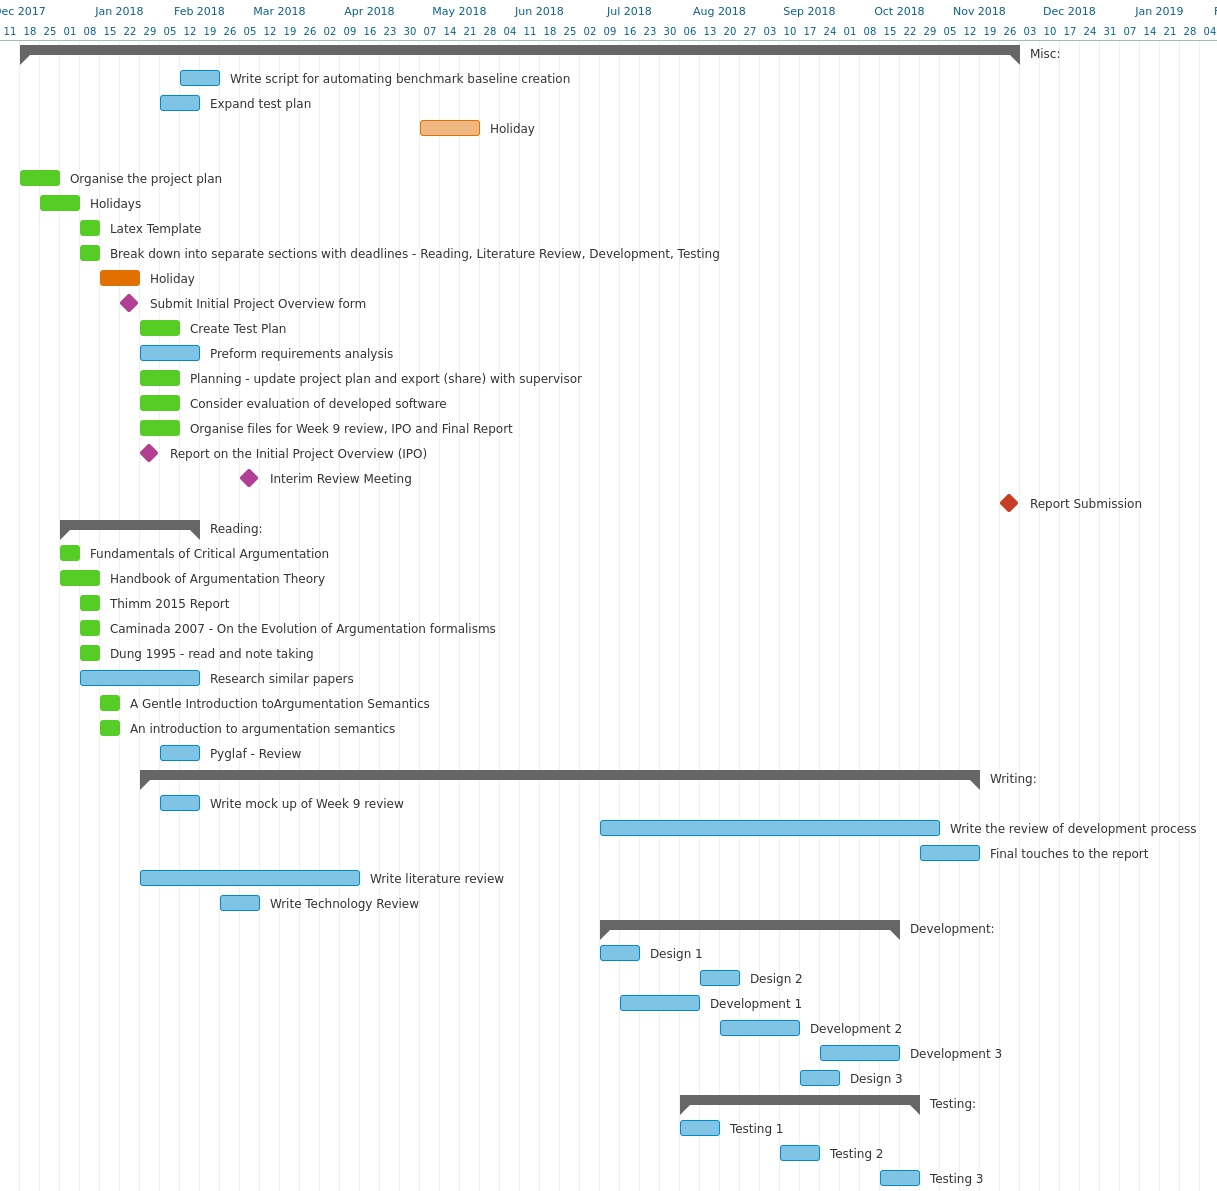
\includegraphics[width=\textwidth]{gantt1}
	\caption{Project Schedule}
	\label{fig:projectSchedule}
\end{figure}

\section{Meetings diaries}
\label{appendix:diaries}
\newpage
\includepdf{./diaries/20180116.pdf}
\includepdf{./diaries/20180123.pdf}
\includepdf{./diaries/20180130.pdf}
\includepdf{./diaries/20180206.pdf}
\includepdf{./diaries/20180213.pdf}
\includepdf{./diaries/20180220.pdf}
\includepdf{./diaries/20181008.pdf}

\section{ICCMA 2017 Submissions}
\label{appendix:ICCMASubmissions}
\begin{center}
\begin{longtable}{| p{.2\textwidth} | p{.8\textwidth} |}
\caption{ICCMA 2017 Submissions}
\label{table:ICCMA2017Submissions}\\

\hline \multicolumn{1}{|c|}{\textbf{Solver}} & \multicolumn{1}{c|}{\textbf{Author}}\\ \hline 
\endfirsthead


\multicolumn{2}{c}%
{{\bfseries \tablename\ \thetable{} -- continued from previous page}} \\
\hline \multicolumn{1}{|c|}{\textbf{Solver}} &
\multicolumn{1}{c|}{\textbf{Author}} \\ \hline 
\endhead

\hline \multicolumn{2}{|r|}{{Continued on next page}} \\ \hline
\endfoot

\hline \hline
\endlastfoot

argmat-clpb   & Fuan Pu (Tsinghua University, China), Guiming Luo (Tsinghua University, China), Yucheng Chen (Tsinghua University, China).                  \\ \midrule
argmat-dvisat & Fuan Pu (Tsinghua University, China), Guiming Luo (Tsinghua University, China), Ya Hang (Tsinghua University, China).                    \\ \hline
argmat-mpg & Fuan Pu (Tsinghua University, China), Guiming Luo (Tsinghua University, China), Ya Hang (Tsinghua University, China).                    \\ \hline
argmat-sat & Fuan Pu (Tsinghua University, China), Guiming Luo (Tsinghua University, China), Ya Hang (Tsinghua University, China).                    \\ \hline
ArgSemSAT  & Federico Cerutti (Cardiff University, UK), Mauro Vallati (University of Huddersfield, UK), Massimiliano Giacomin (University of Brescia, Italy), Tobia Zanetti (University of Brescia, Italy). \\ \hline
ArgTools   & Samer Nofal (German Jordanian University, Jordan), Katie Atkinson (University of Liverpool, UK), Paul E. Dunne (University of Liverpool, UK).              \\ \hline
ASPrMin    & Wolfgang Faber (University of Huddersfield, UK), Mauro Vallati (University of Huddersfield, UK), Federico Cerutti (Cardiff University, UK), Massimiliano Giacomin (University of Brescia, Italy). \\ \hline
cegartix   & Wolfgang Dvořák (TU Wien, Austria), Matti Järvisalo (University of Helsinki, Finland), Johannes P. Wallner (TU Wien, Austria).                 \\ \hline
Chimærarg  & Federico Cerutti (Cardiff University, UK), Mauro Vallati (University of Huddersfield, UK), Massimiliano Giacomin (University of Brescia, Italy).              \\ \hline
ConArg  & Stefano Bistarelli (Università di Perugia, Italy), Fabio Rossi (Università di Perugia, Italy), Francesco Santini (Università di Perugia, Italy).              \\ \hline
CoQuiAAS   & Jean-Marie Lagniez (Univ. Artois, France), Emmanuel Lonca (Univ. Artois, France), Jean-Guy Mailly (Univ. Paris Descartes, France).                \\ \hline
EqArgSolver   & Odinaldo Rodrigues (King's College London, UK).                                       \\ \hline
gg-sts  & Tomi Jahunen (Aalto University, Finland), Shahab Tasharrofi (Aalto University, Finland).                            \\ \hline
goDIAMOND  & Stefan Ellmauthaler (Leipzig University, Germany), Hannes Strass (Leipzig University, Germany).                           \\ \hline
heureka    & Nils Geilen (Universität Koblenz-Landau, Germany), Matthias Thimm (Universität Koblenz-Landau, Germany).                        \\ \hline
pyglaf  & Mario Alviano (University of Calabria, Italy).                                       
\end{longtable}
\end{center}


\section{Argumentation Framework Graph}
\label{appendix:aficcma}
\begin{figure}
	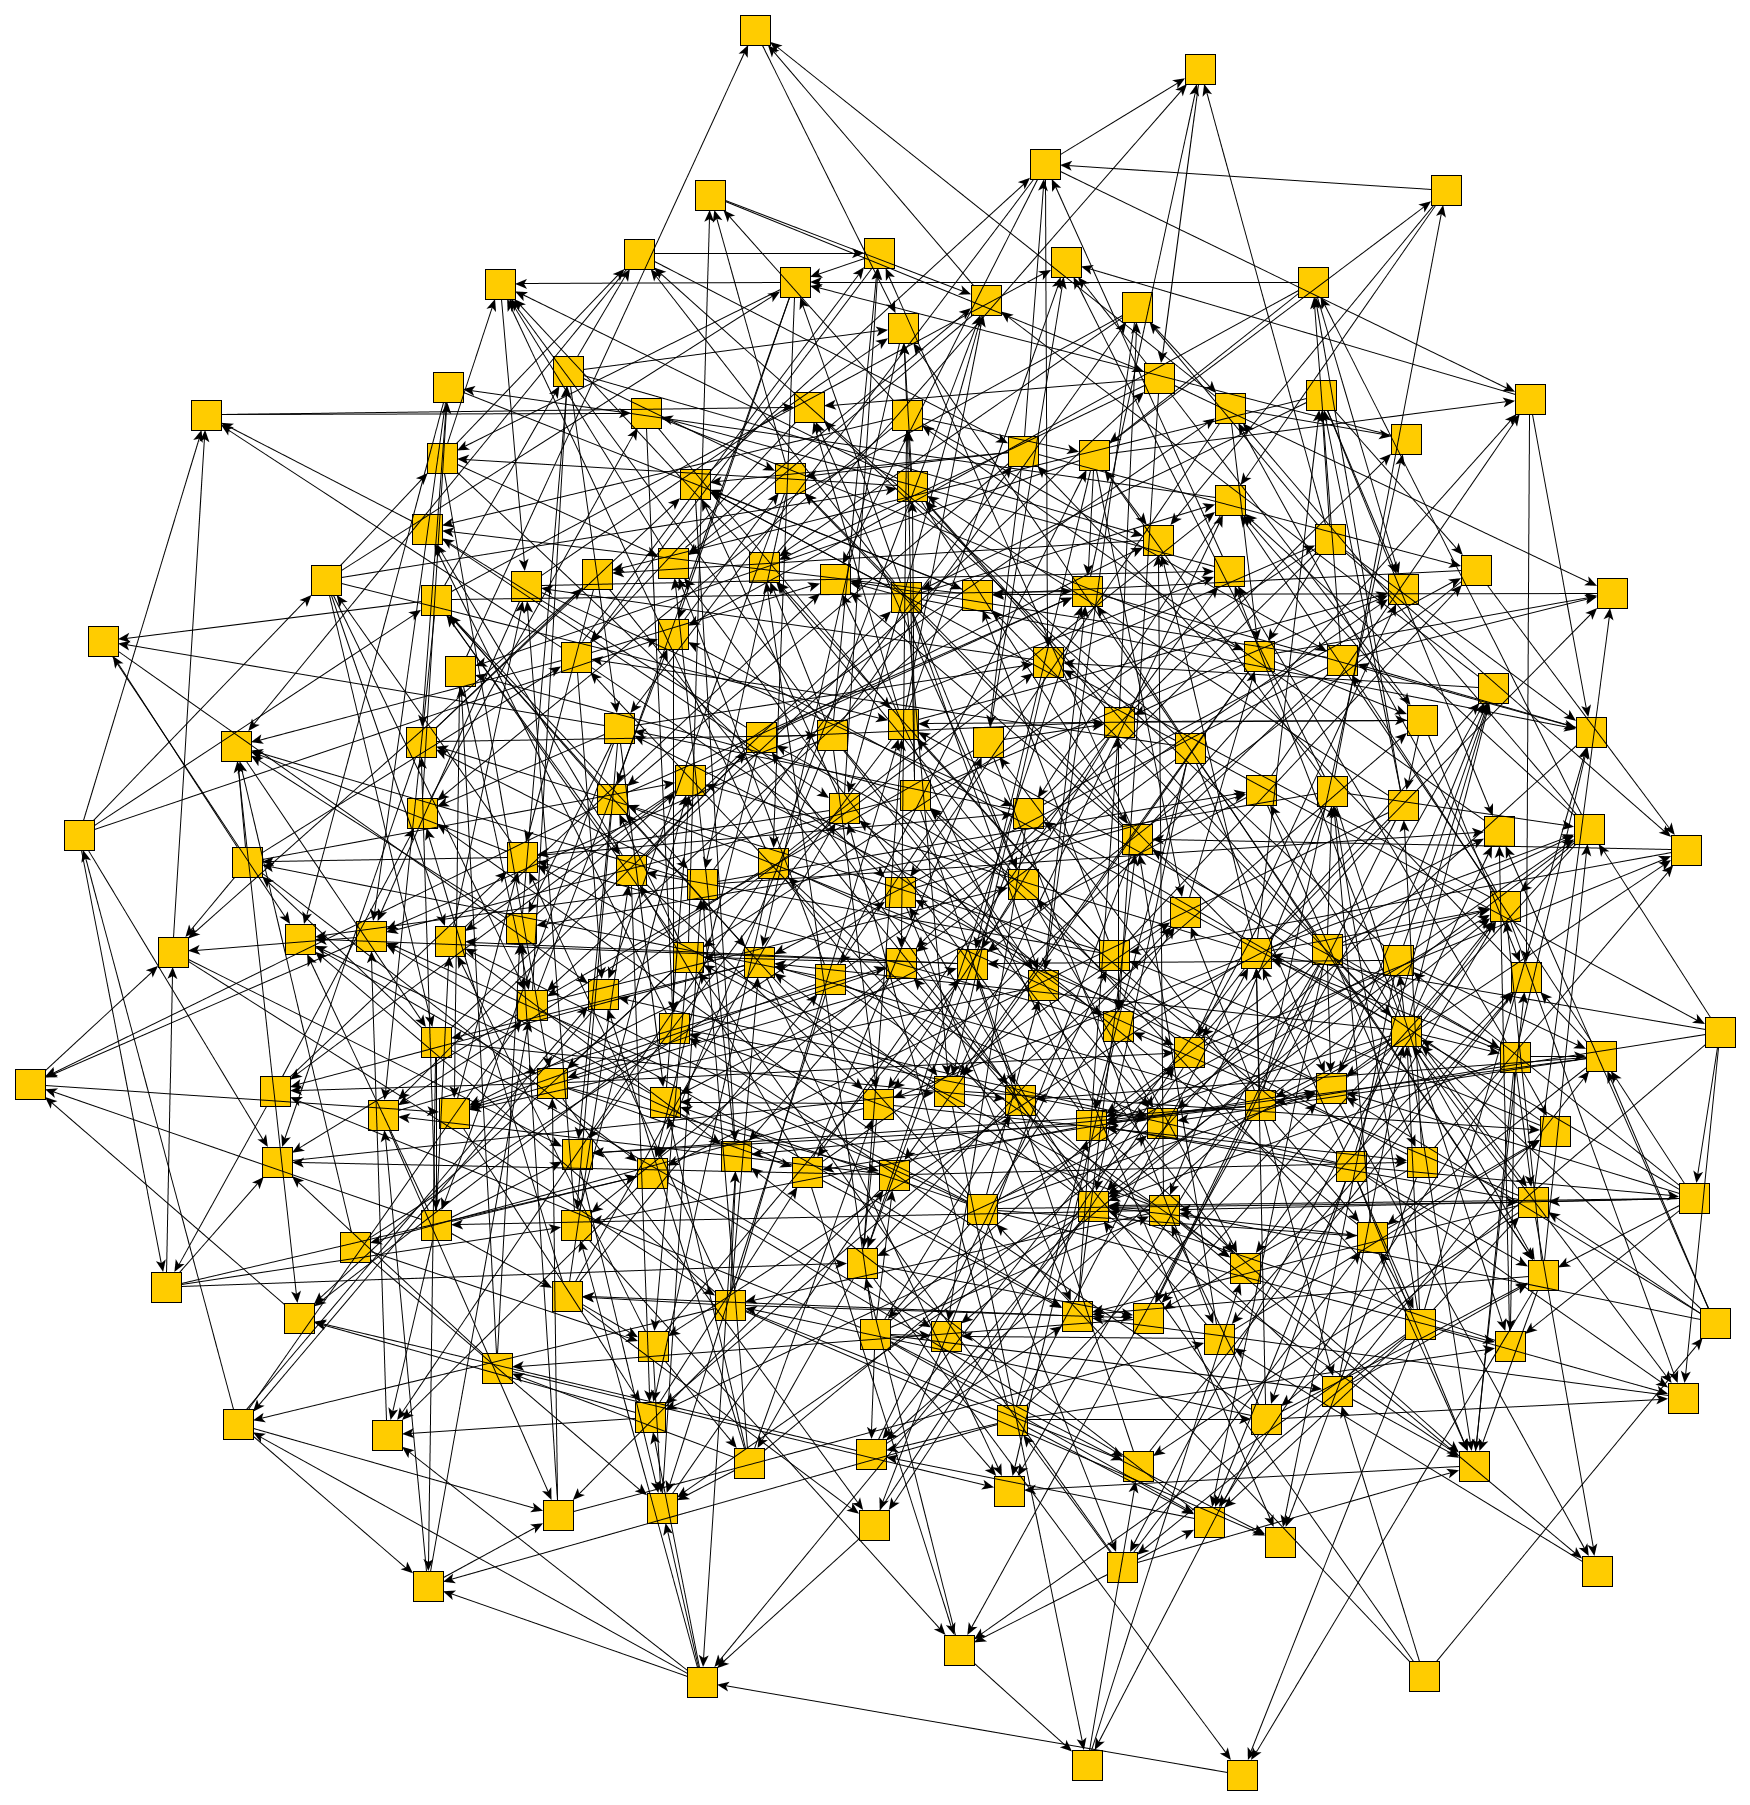
\includegraphics[width=0.9\textwidth]{AFICCMA}
	\caption{Example argumentation framework graph}
\end{figure}

\section{Benchmark Files}
\label{appendix:benchmarkFiles}

\begin{longtable}{| p{.8\textwidth} | p{.1\textwidth} | p{.1\textwidth} | }
	\caption{Benchmark Files for Stable Extensions}
	\label{table:stableFiles} \\
	
	
\hline
Filename                                                             & Args & Attacks \\ \hline
massachusetts\_blockislandferry\_2015-11-13.gml.80.tgf               & 2         & 1       \\
test.tgf                                                             & 6         & 10      \\
university-of-pretoria\_20150805\_1406.normalized.gml.80.tgf         & 13        & 17      \\
afinput\_exp\_cycles\_indvary3\_step4\_batch\_yyy03.tgf              & 15        & 5       \\
afinput\_exp\_acyclic\_indvary3\_step7\_batch\_yyy01.tgf             & 15        & 2       \\
massachusetts-archiver\_20090912\_0208.gml.50.tgf                    & 34        & 58      \\
BA\_40\_80\_4.tgf                                                    & 41        & 73      \\
BA\_40\_30\_3.tgf                                                    & 41        & 53      \\
BA\_40\_60\_2.tgf                                                    & 41        & 65      \\
afinput\_exp\_cycles\_indvary1\_step8\_batch\_yyy08.tgf              & 41        & 216     \\
sembuster\_60.tgf                                                    & 60        & 460     \\
afinput\_exp\_acyclic\_indvary1\_step3\_batch\_yyy06.tgf             & 74        & 3427    \\
ER\_100\_50\_6.tgf                                                   & 101       & 2489    \\
ER\_100\_20\_8.tgf                                                   & 101       & 955     \\
BA\_100\_20\_1.tgf                                                   & 101       & 121     \\
BA\_120\_20\_2.tgf                                                   & 121       & 145     \\
stb\_138\_162.tgf                                                    & 138       & 1391    \\
grd\_156\_3\_6.tgf                                                   & 156       & 409     \\
ferry2.pfile-L2-C1-02.pddl.2.cnf.tgf                                 & 160       & 279     \\
stb\_161\_74.tgf                                                     & 161       & 1400    \\
stb\_199\_128.tgf                                                    & 199       & 442     \\
WS\_200\_14\_30\_70.tgf                                              & 200       & 1400    \\
ferry2.pfile-L2-C2-06.pddl.2.cnf.tgf                                 & 239       & 432     \\
stb\_245\_206.tgf                                                    & 245       & 649     \\
ferry2.pfile-L2-C2-08.pddl.2.cnf.tgf                                 & 276       & 500     \\
ER\_300\_100\_7.tgf                                                  & 302       & 45305   \\
scc\_359\_50\_5\_17.tgf                                              & 359       & 2657    \\
ferry2.pfile-L3-C1-04.pddl.3.cnf.tgf                                 & 373       & 647     \\
afinput\_exp\_acyclic\_depvary\_step5\_batch\_yyy08.tgf              & 384       & 133973  \\
WS\_400\_8\_30\_30.tgf                                               & 400       & 1600    \\
WS\_400\_8\_10\_70.tgf                                               & 400       & 1600    \\
WS\_400\_8\_70\_10.tgf                                               & 400       & 1600    \\
ER\_400\_100\_8.tgf                                                  & 402       & 80398   \\
ER\_400\_100\_9.tgf                                                  & 402       & 80386   \\
scc\_411\_40\_10\_23.tgf                                             & 411       & 5165    \\
WS\_500\_8\_50\_70.tgf                                               & 500       & 2000    \\
sembuster\_600.tgf                                                   & 600       & 40600   \\
scc\_669\_70\_10\_21.tgf                                             & 669       & 20208   \\
ferry2.pfile-L2-C4-07.pddl.3.cnf.tgf                                 & 754       & 1336    \\
scc\_874\_30\_20\_25.tgf                                             & 874       & 28768   \\
sembuster\_900.tgf                                                   & 900       & 90900   \\
empresa-publica-de-transportes-e-circulao\_20141104\_0243.gml.20.tgf & 930       & 2577    \\
admbuster\_1000.tgf                                                  & 1000      & 1498    \\
sembuster\_1200.tgf                                                  & 1200      & 161200  \\
grd\_1892\_1\_3.tgf                                                  & 1892      & 17773   \\
grd\_1948\_5\_1.tgf                                                  & 1948      & 94841   \\
admbuster\_2000.tgf                                                  & 2000      & 2998    \\
omnitrans\_20151217\_1124.gml.20.tgf                                 & 2188      & 3028    \\
grd\_3018\_3\_7.tgf                                                  & 3018      & 137019  \\
admbuster\_20000.tgf                                                 & 20000     & 29998   \\
admbuster\_50000.tgf                                                 & 50000     & 74998  
\end{longtable}


\begin{longtable}{| p{.8\textwidth} | p{.1\textwidth} | p{.1\textwidth} | }
	\caption{Benchmark Files for Preferred and Complete Extensions}
	\label{table:prefFiles} \\
	
	\hline
	Filename                                                                       & Args & Attacks \\ \hline
	massachusetts\_vineyardfastferry\_2015-11-13.gml.50.tgf                        & 3    & 2       \\
	hut-airport-shuttle\_20120105\_0729.gml.50.tgf                                 & 7    & 7       \\
	brookings-or-us.gml.50.tgf                                                     & 12   & 18      \\
	afinput\_exp\_cycles\_indvary3\_step8\_batch\_yyy07.tgf                        & 15   & 1       \\
	rockland-county-department-of-public-transportation\_20121220\_2018.gml.20.tgf & 16   & 30      \\
	caravan-or-us.gml.80.tgf                                                       & 19   & 37      \\
	afinput\_exp\_acyclic\_indvary1\_step5\_batch\_yyy04.tgf                       & 26   & 90      \\
	afinput\_exp\_acyclic\_indvary3\_step1\_batch\_yyy10.tgf                       & 30   & 85      \\
	afinput\_exp\_acyclic\_indvary1\_step5\_batch\_yyy09.tgf                       & 41   & 543     \\
	BA\_40\_80\_5.tgf                                                              & 41   & 73      \\
	afinput\_exp\_acyclic\_depvary\_step3\_batch\_yyy01.tgf                        & 50   & 1478    \\
	sembuster\_60.tgf                                                              & 60   & 460     \\
	BA\_60\_70\_3.tgf                                                              & 61   & 102     \\
	ferry2.pfile-L2-C1-08.pddl.1.cnf.tgf                                           & 86   & 136     \\
	WS\_100\_6\_70\_30.tgf                                                         & 100  & 300     \\
	WS\_100\_18\_30\_10.tgf                                                        & 100  & 900     \\
	WS\_100\_12\_10\_70.tgf                                                        & 100  & 600     \\
	WS\_100\_12\_50\_30.tgf                                                        & 100  & 600     \\
	ER\_100\_50\_6.tgf                                                             & 101  & 2489    \\
	ER\_100\_90\_4.tgf                                                             & 101  & 4556    \\
	ER\_100\_100\_1.tgf                                                            & 102  & 5094    \\
	BA\_120\_30\_3.tgf                                                             & 121  & 157     \\
	ferry2.pfile-L2-C2-08.pddl.1.cnf.tgf                                           & 135  & 220     \\
	sembuster\_150.tgf                                                             & 150  & 2650    \\
	BA\_180\_10\_2.tgf                                                             & 181  & 199     \\
	stb\_190\_70.tgf                                                               & 190  & 821     \\
	stb\_196\_281.tgf                                                              & 196  & 2384    \\
	BA\_200\_10\_5.tgf                                                             & 201  & 221     \\
	ER\_200\_70\_5.tgf                                                             & 201  & 14053   \\
	ferry2.pfile-L2-C1-05.pddl.3.cnf.tgf                                           & 205  & 334     \\
	ferry2.pfile-L3-C1-04.pddl.2.cnf.tgf                                           & 273  & 507     \\
	stb\_291\_2.tgf                                                                & 291  & 3361    \\
	ER\_300\_100\_4.tgf                                                            & 302  & 45313   \\
	scc\_341\_30\_5\_9.tgf                                                         & 341  & 2715    \\
	stb\_389\_42.tgf                                                               & 389  & 1652    \\
	grd\_418\_2\_9.tgf                                                             & 418  & 1747    \\
	stb\_437\_137.tgf                                                              & 437  & 1539    \\
	grd\_489\_5\_8.tgf                                                             & 489  & 5944    \\
	WS\_500\_16\_30\_70.tgf                                                        & 500  & 4000    \\
	ferry2.pfile-L3-C2-02.pddl.2.cnf.tgf                                           & 528  & 1012    \\
	scc\_845\_40\_5\_19.tgf                                                        & 845  & 11331   \\
	scc\_989\_70\_15\_3.tgf                                                        & 989  & 42499   \\
	admbuster\_1000.tgf                                                            & 1000 & 1498    \\
	scc\_1109\_50\_10\_5.tgf                                                       & 1109 & 33830   \\
	scc\_1439\_40\_15\_17.tgf                                                      & 1439 & 63081   \\
	grd\_1790\_4\_8.tgf                                                            & 1790 & 64086   \\
	admbuster\_2000.tgf                                                            & 2000 & 2998    \\
	grd\_2065\_1\_8.tgf                                                            & 2065 & 21185   \\
	admbuster\_4000.tgf                                                            & 4000 & 5998    \\
	admbuster\_6000.tgf                                                            & 6000 & 8998   
\end{longtable}

\section{Stable Extension Testing Results}
\label{appendix:stableResults}
% Please add the following required packages to your document preamble:
% \usepackage{booktabs}
%
\begin{landscape}
\begin{longtabu} {|l|l|l|l|l|l|l|l|}
\toprule
Args & Att & Sets     & PyTables & Parallel Dicts & SAT      & pyglaf      & argsem-sat  \\ \midrule
\endhead

2         & 1       & 0.000453 & 0.00279  & 0.000326395    & 0.009292 & 0.065012217 & 0.025399447 \\
6         & 10      & 0.000871 & 0.024364 & 0.000370264    & 0.000291 & 0.06543088  & 0.007328749 \\
13        & 17      & 0.006193 & 19.4888  & 0.001136303    & 0.003224 & 0.064931393 & 0.006547213 \\
15        & 5       & 0.001764 & 0.174153 & 0.000958681    & 0.000108 & 0.065138578 & 0.006511688 \\
15        & 2       & 0.000605 & 0.012517 & 0.000642538    & 8.42E-05 & 0.065627575 & 0.005755186 \\
34        & 58      & 27.70923 & Time out & 6.216353655    & Time out & 0.071168423 & 0.098623753 \\
41        & 73      & 12.69499 & Time out & 0.093905449    & Time out & 0.078179121 & 0.016719103 \\
41        & 53      & 9.555216 & Time out & 0.324863195    & Time out & 0.064435959 & 0.010287523 \\
41        & 65      & 2.930374 & Time out & 0.01935029     & Time out & 0.067563057 & 0.010713577 \\
41        & 216     & 0.028529 & Time out & 0.003152132    & 0.001259 & 0.066415548 & 0.006392717 \\
60        & 460     & 5.29241  & Time out & 0.00635314     & Time out & 0.068720818 & 0.009454727 \\
74        & 3427    & 40.53372 & Time out & 0.052899837    & 0.008584 & 0.085255146 & 0.055872917 \\
101       & 2489    & Time out & Time out & 369.106797     & 888.5523 & 0.104641676 & 0.036447287 \\
101       & 955     & Time out & Time out & Time out       & Time out & 0.074910879 & 0.017008066 \\
101       & 121     & Time out & Time out & Time out       & Time out & 0.068510771 & 0.036782265 \\
121       & 145     & Time out & Time out & Time out       & Time out & 0.069716692 & 0.03000617  \\
138       & 1391    & Time out & Time out & Time out       & Time out & 0.081300974 & 0.018036366 \\
156       & 409     & Time out & Time out & Time out       & Time out & 0.069542408 & 0.009888887 \\
160       & 279     & Time out & Time out & Time out       & Time out & 0.068692446 & 0.031356812 \\
161       & 1400    & Time out & Time out & Time out       & Time out & 0.080003738 & 0.02195406  \\
199       & 442     & Time out & Time out & Time out       & Time out & 0.069525242 & 0.012038708 \\
200       & 1400    & Time out & Time out & Time out       & Time out & 0.080610275 & 0.015025139 \\
239       & 432     & Time out & Time out & Time out       & Time out & 0.072205782 & 0.021214247 \\
245       & 649     & Time out & Time out & Time out       & Time out & 0.071638107 & 0.010595083 \\
276       & 500     & Time out & Time out & Time out       & Time out & 0.069832802 & 0.027677298 \\
302       & 45305   & Time out & Time out & 1.278002739    & 0.184559 & 4.159725905 & 1.220250845 \\
359       & 2657    & Time out & Time out & Time out       & Time out & 0.081829548 & 0.017944336 \\
373       & 647     & Time out & Time out & Time out       & Time out & 0.078984261 & 0.136862278 \\
384       & 133973  & Time out & Time out & 1.474908352    & 1.644092 & 0.965767145 & 7.981366396 \\
400       & 1600    & Time out & Time out & Time out       & Time out & 0.083271503 & 0.014073849 \\
400       & 1600    & Time out & Time out & Time out       & Time out & 0.079077721 & 0.014715433 \\
400       & 1600    & Time out & Time out & Time out       & Time out & 0.093198299 & 0.034980297 \\
402       & 80398   & Time out & Time out & 2.609353781    & 0.364464 & 12.10009837 & 2.795321226 \\
402       & 80386   & Time out & Time out & 2.742642164    & 0.364939 & 12.14501143 & 2.850753784 \\
411       & 5165    & Time out & Time out & Time out       & Time out & 0.101779223 & 0.043988705 \\
500       & 2000    & Time out & Time out & Time out       & Time out & 0.089668989 & 0.019552231 \\
600       & 40600   & Time out & Time out & 3.640912294    & Time out & 1.352958679 & 1.048346758 \\
669       & 20208   & Time out & Time out & Time out       & Time out & 0.228774309 & 0.173240423 \\
754       & 1336    & Time out & Time out & Time out       & Time out & 0.089713812 & 0.121773958 \\
874       & 28768   & Time out & Time out & Time out       & Time out & 0.268687725 & 0.282220125 \\
900       & 90900   & Time out & Time out & 14.70816398    & Time out & 6.464350939 & 3.204070091 \\
930       & 2577    & Time out & Time out & Time out       & Time out & 0.088249922 & 0.020265579 \\
1000      & 1498    & Time out & Time out & Time out       & Time out & 0.083356857 & 0.021613836 \\
1200      & 161200  & Time out & Time out & 42.30723596    & Time out & 16.23498964 & 7.5222013   \\
1892      & 17773   & Time out & Time out & Time out       & Time out & 0.230313778 & 0.133599758 \\
1948      & 94841   & Time out & Time out & Time out       & Time out & 1.47881341  & 1.372130632 \\
2000      & 2998    & Time out & Time out & Time out       & Time out & 0.110507488 & 0.038184404 \\
2188      & 3028    & Time out & Time out & Time out       & Time out & 0.107483864 & 0.030617476 \\
3018      & 137019  & Time out & Time out & Time out       & Time out & 2.199171305 & 2.013922215 \\
20000     & 29998   & Time out & Time out & Time out       & Time out & 0.539016247 & 0.395638228 \\
50000     & 74998   & Time out & Time out & Time out       & Time out & 1.365074396 & 0.93032527  \\ \bottomrule
\end{longtabu}
\end{landscape}
%\begin{subappendices}
%\subsection{Example sub appendices}
...
%\end{subappendices}

%\section{Second Formal Review Output}
%Insert a copy of the project review form you were given at the end of the review by %the second marker

%\section{Diary Sheets (or other project management evidence)}
%Insert diary sheets here together with any project management plan you have

%\section{Appendix 4 and following}
%insert content here and for each of the other appendices, the title may be just on a page by itself, the pages of the appendices are not numbered, unless an included document such as a user manual or design document is itself pager numbered.
\end{appendices}

\end{document}
